% **************************************************************************************************************
% A Classic Thesis Style
% An Homage to The Elements of Typographic Style
%
% Copyright (C) 2015 André Miede http://www.miede.de
%
% If you like the style then I would appreciate a postcard. My address 
% can be found in the file ClassicThesis.pdf. A collection of the 
% postcards I received so far is available online at 
% http://postcards.miede.de
%
% License:
% This program is free software; you can redistribute it and/or modify
% it under the terms of the GNU General Public License as published by
% the Free Software Foundation; either version 2 of the License, or
% (at your option) any later version.
%
% This program is distributed in the hope that it will be useful,
% but WITHOUT ANY WARRANTY; without even the implied warranty of
% MERCHANTABILITY or FITNESS FOR A PARTICULAR PURPOSE.  See the
% GNU General Public License for more details.
%
% You should have received a copy of the GNU General Public License
% along with this program; see the file COPYING.  If not, write to
% the Free Software Foundation, Inc., 59 Temple Place - Suite 330,
% Boston, MA 02111-1307, USA.
%
% **************************************************************************************************************
\RequirePackage{fix-cm} % fix some latex issues see: http://texdoc.net/texmf-dist/doc/latex/base/fixltx2e.pdf
\documentclass[ twoside,openright,titlepage,numbers=noenddot,headinclude,%1headlines,% letterpaper a4paper
                footinclude=true,cleardoublepage=empty,abstractoff, % <--- obsolete, remove (todo)
                BCOR=5mm,paper=a4,fontsize=14pt,%11pt,a4paper,%
                ngerman,american,%
                ]{scrreprt}

\usepackage[strict]{changepage}% <-- new
\usepackage{booktabs,tabularx}% <-- added that your MWE can be compiled
\usepackage{blindtext}
%********************************************************************
% Note: Make all your adjustments in here
%*******************************************************
% ****************************************************************************************************
% classicthesis-config.tex 
% formerly known as loadpackages.sty, classicthesis-ldpkg.sty, and classicthesis-preamble.sty 
% Use it at the beginning of your ClassicThesis.tex, or as a LaTeX Preamble 
% in your ClassicThesis.{tex,lyx} with % ****************************************************************************************************
% classicthesis-config.tex 
% formerly known as loadpackages.sty, classicthesis-ldpkg.sty, and classicthesis-preamble.sty 
% Use it at the beginning of your ClassicThesis.tex, or as a LaTeX Preamble 
% in your ClassicThesis.{tex,lyx} with % ****************************************************************************************************
% classicthesis-config.tex 
% formerly known as loadpackages.sty, classicthesis-ldpkg.sty, and classicthesis-preamble.sty 
% Use it at the beginning of your ClassicThesis.tex, or as a LaTeX Preamble 
% in your ClassicThesis.{tex,lyx} with \input{classicthesis-config}
% ****************************************************************************************************  
% If you like the classicthesis, then I would appreciate a postcard. 
% My address can be found in the file ClassicThesis.pdf. A collection 
% of the postcards I received so far is available online at 
% http://postcards.miede.de
% ****************************************************************************************************


% ****************************************************************************************************
% 0. Set the encoding of your files. UTF-8 is the only sensible encoding nowadays. If you can't read
% äöüßáéçèê∂åëæƒÏ€ then change the encoding setting in your editor, not the line below. If your editor
% does not support utf8 use another editor!
% ****************************************************************************************************
\PassOptionsToPackage{utf8}{inputenc}
	\usepackage{inputenc}

% ****************************************************************************************************
% 1. Configure classicthesis for your needs here, e.g., remove "drafting" below 
% in order to deactivate the time-stamp on the pages
% ****************************************************************************************************
\PassOptionsToPackage{eulerchapternumbers,listings,%
					 pdfspacing,%floatperchapter,%linedheaders,%
					 subfig,beramono,eulermath,parts}{classicthesis}                                        
% ********************************************************************
% Available options for classicthesis.sty 
% (see ClassicThesis.pdf for more information):
% drafting
% parts nochapters linedheaders
% eulerchapternumbers beramono eulermath pdfspacing minionprospacing
% tocaligned dottedtoc manychapters
% listings floatperchapter subfig
% ********************************************************************


% ****************************************************************************************************
% 2. Personal data and user ad-hoc commands
% ****************************************************************************************************
\newcommand{\myTitle}{Night-time lights as a proxy for economic variables\xspace}
\newcommand{\mySubtitle}{subtitle\xspace}
\newcommand{\myDegree}{Doktor-Ingenieur (Dr.-Ing.)\xspace}
\newcommand{\myName}{Nicolò Badino\xspace}
\newcommand{\myProf}{Federico Crudu\xspace}
\newcommand{\myOtherProf}{Put name here\xspace}
\newcommand{\mySupervisor}{Put name here\xspace}
\newcommand{\myFaculty}{Put data here\xspace}
\newcommand{\myDepartment}{Put data here\xspace}
\newcommand{\myUni}{Put data here\xspace}
\newcommand{\myLocation}{Saarbrücken\xspace}
\newcommand{\myTime}{September 2015\xspace}
\newcommand{\myVersion}{version 4.2\xspace}

% ********************************************************************
% Setup, finetuning, and useful commands
% ********************************************************************
\newcounter{dummy} % necessary for correct hyperlinks (to index, bib, etc.)
\newlength{\abcd} % for ab..z string length calculation
\providecommand{\mLyX}{L\kern-.1667em\lower.25em\hbox{Y}\kern-.125emX\@}
\newcommand{\ie}{i.\,e.}
\newcommand{\Ie}{I.\,e.}
\newcommand{\eg}{e.\,g.}
\newcommand{\Eg}{E.\,g.} 
% ****************************************************************************************************


% ****************************************************************************************************
% 3. Loading some handy packages
% ****************************************************************************************************
% ******************************************************************** 
% Packages with options that might require adjustments
% ******************************************************************** 
%\PassOptionsToPackage{ngerman,american}{babel}   % change this to your language(s)
% Spanish languages need extra options in order to work with this template
%\PassOptionsToPackage{spanish,es-lcroman}{babel}
	\usepackage{babel}                  

\usepackage{csquotes}
\PassOptionsToPackage{%
    %backend=biber, %instead of bibtex
	backend=bibtex8,bibencoding=ascii,%
	language=auto,%
	style=numeric-comp,%
    style=authoryear-comp, % Author 1999, 2010
    bibstyle=authoryear,dashed=false, % dashed: substitute rep. author with ---
    sorting=nyt, % name, year, title
    maxbibnames=10, % default: 3, et al.
    %backref=true,%
    natbib=true % natbib compatibility mode (\citep and \citet still work)
}{biblatex}
    \usepackage{biblatex}

\PassOptionsToPackage{fleqn}{amsmath}       % math environments and more by the AMS 
    \usepackage{amsmath}

% ******************************************************************** 
% General useful packages
% ******************************************************************** 
\PassOptionsToPackage{T1}{fontenc} % T2A for cyrillics
    \usepackage{fontenc}     
\usepackage{textcomp} % fix warning with missing font shapes
\usepackage{scrhack} % fix warnings when using KOMA with listings package          
\usepackage{xspace} % to get the spacing after macros right  
\usepackage{mparhack} % get marginpar right
\usepackage{fixltx2e} % fixes some LaTeX stuff --> since 2015 in the LaTeX kernel (see below)
%\usepackage[latest]{latexrelease} % will be used once available in more distributions (ISSUE #107)
\PassOptionsToPackage{printonlyused,smaller}{acronym} 
    \usepackage{acronym} % nice macros for handling all acronyms in the thesis
    %\renewcommand{\bflabel}[1]{{#1}\hfill} % fix the list of acronyms --> no longer working
    %\renewcommand*{\acsfont}[1]{\textsc{#1}} 
    \renewcommand*{\aclabelfont}[1]{\acsfont{#1}}
% ****************************************************************************************************


% ****************************************************************************************************
% 4. Setup floats: tables, (sub)figures, and captions
% ****************************************************************************************************
\usepackage{tabularx} % better tables
    \setlength{\extrarowheight}{3pt} % increase table row height
\newcommand{\tableheadline}[1]{\multicolumn{1}{c}{\spacedlowsmallcaps{#1}}}
\newcommand{\myfloatalign}{\centering} % to be used with each float for alignment
\usepackage{caption}
% Thanks to cgnieder and Claus Lahiri
% http://tex.stackexchange.com/questions/69349/spacedlowsmallcaps-in-caption-label
% [REMOVED DUE TO OTHER PROBLEMS, SEE ISSUE #82]    
%\DeclareCaptionLabelFormat{smallcaps}{\bothIfFirst{#1}{~}\MakeTextLowercase{\textsc{#2}}}
%\captionsetup{font=small,labelformat=smallcaps} % format=hang,
\captionsetup{font=small} % format=hang,
\usepackage{subfig}  
% ****************************************************************************************************


% ****************************************************************************************************
% 5. Setup code listings
% ****************************************************************************************************
\usepackage{listings} 
%\lstset{emph={trueIndex,root},emphstyle=\color{BlueViolet}}%\underbar} % for special keywords
\lstset{language=[LaTeX]Tex,%C++,
    morekeywords={PassOptionsToPackage,selectlanguage},
    keywordstyle=\color{RoyalBlue},%\bfseries,
    basicstyle=\small\ttfamily,
    %identifierstyle=\color{NavyBlue},
    commentstyle=\color{Green}\ttfamily,
    stringstyle=\rmfamily,
    numbers=none,%left,%
    numberstyle=\scriptsize,%\tiny
    stepnumber=5,
    numbersep=8pt,
    showstringspaces=false,
    breaklines=true,
    %frameround=ftff,
    %frame=single,
    belowcaptionskip=.75\baselineskip
    %frame=L
} 
% ****************************************************************************************************             


% ****************************************************************************************************
% 6. PDFLaTeX, hyperreferences and citation backreferences
% ****************************************************************************************************
% ********************************************************************
% Using PDFLaTeX
% ********************************************************************
\PassOptionsToPackage{pdftex,hyperfootnotes=false,pdfpagelabels}{hyperref}
    \usepackage{hyperref}  % backref linktocpage pagebackref
\pdfcompresslevel=9
\pdfadjustspacing=1 
\PassOptionsToPackage{pdftex}{graphicx}
    \usepackage{graphicx} 
 

% ********************************************************************
% Hyperreferences
% ********************************************************************
\hypersetup{%
    %draft, % = no hyperlinking at all (useful in b/w printouts)
    colorlinks=true, linktocpage=true, pdfstartpage=3, pdfstartview=FitV,%
    % uncomment the following line if you want to have black links (e.g., for printing)
    %colorlinks=false, linktocpage=false, pdfstartpage=3, pdfstartview=FitV, pdfborder={0 0 0},%
    breaklinks=true, pdfpagemode=UseNone, pageanchor=true, pdfpagemode=UseOutlines,%
    plainpages=false, bookmarksnumbered, bookmarksopen=true, bookmarksopenlevel=1,%
    hypertexnames=true, pdfhighlight=/O,%nesting=true,%frenchlinks,%
    urlcolor=webbrown, linkcolor=RoyalBlue, citecolor=webgreen, %pagecolor=RoyalBlue,%
    %urlcolor=Black, linkcolor=Black, citecolor=Black, %pagecolor=Black,%
    pdftitle={\myTitle},%
    pdfauthor={\textcopyright\ \myName, \myUni, \myFaculty},%
    pdfsubject={},%
    pdfkeywords={},%
    pdfcreator={pdfLaTeX},%
    pdfproducer={LaTeX with hyperref and classicthesis}%
}   

% ********************************************************************
% Setup autoreferences
% ********************************************************************
% There are some issues regarding autorefnames
% http://www.ureader.de/msg/136221647.aspx
% http://www.tex.ac.uk/cgi-bin/texfaq2html?label=latexwords
% you have to redefine the makros for the 
% language you use, e.g., american, ngerman
% (as chosen when loading babel/AtBeginDocument)
% ********************************************************************
\makeatletter
\@ifpackageloaded{babel}%
    {%
       \addto\extrasamerican{%
			\renewcommand*{\figureautorefname}{Figure}%
			\renewcommand*{\tableautorefname}{Table}%
			\renewcommand*{\partautorefname}{Part}%
			\renewcommand*{\chapterautorefname}{Chapter}%
			\renewcommand*{\sectionautorefname}{Section}%
			\renewcommand*{\subsectionautorefname}{Section}%
			\renewcommand*{\subsubsectionautorefname}{Section}%     
                }%
       \addto\extrasngerman{% 
			\renewcommand*{\paragraphautorefname}{Absatz}%
			\renewcommand*{\subparagraphautorefname}{Unterabsatz}%
			\renewcommand*{\footnoteautorefname}{Fu\"snote}%
			\renewcommand*{\FancyVerbLineautorefname}{Zeile}%
			\renewcommand*{\theoremautorefname}{Theorem}%
			\renewcommand*{\appendixautorefname}{Anhang}%
			\renewcommand*{\equationautorefname}{Gleichung}%        
			\renewcommand*{\itemautorefname}{Punkt}%
                }%  
            % Fix to getting autorefs for subfigures right (thanks to Belinda Vogt for changing the definition)
            \providecommand{\subfigureautorefname}{\figureautorefname}%             
    }{\relax}
\makeatother


% ****************************************************************************************************
% 7. Last calls before the bar closes
% ****************************************************************************************************
% ********************************************************************
% Development Stuff
% ********************************************************************
\listfiles
%\PassOptionsToPackage{l2tabu,orthodox,abort}{nag}
%   \usepackage{nag}
%\PassOptionsToPackage{warning, all}{onlyamsmath}
%   \usepackage{onlyamsmath}

% ********************************************************************
% Last, but not least...
% ********************************************************************
\usepackage{classicthesis} 
% ****************************************************************************************************


% ****************************************************************************************************
% 8. Further adjustments (experimental)
% ****************************************************************************************************
% ********************************************************************
% Changing the text area
% ********************************************************************
%\linespread{1.05} % a bit more for Palatino
%\areaset[current]{312pt}{761pt} % 686 (factor 2.2) + 33 head + 42 head \the\footskip
%\setlength{\marginparwidth}{7em}%
%\setlength{\marginparsep}{2em}%

% ********************************************************************
% Using different fonts
% ********************************************************************
%\usepackage[oldstylenums]{kpfonts} % oldstyle notextcomp
%\usepackage[osf]{libertine}
%\usepackage[light,condensed,math]{iwona}
%\renewcommand{\sfdefault}{iwona}
%\usepackage{lmodern} % <-- no osf support :-(
%\usepackage{cfr-lm} % 
%\usepackage[urw-garamond]{mathdesign} <-- no osf support :-(
%\usepackage[default,osfigures]{opensans} % scale=0.95 
%\usepackage[sfdefault]{FiraSans}
% ****************************************************************************************************

% ****************************************************************************************************  
% If you like the classicthesis, then I would appreciate a postcard. 
% My address can be found in the file ClassicThesis.pdf. A collection 
% of the postcards I received so far is available online at 
% http://postcards.miede.de
% ****************************************************************************************************


% ****************************************************************************************************
% 0. Set the encoding of your files. UTF-8 is the only sensible encoding nowadays. If you can't read
% äöüßáéçèê∂åëæƒÏ€ then change the encoding setting in your editor, not the line below. If your editor
% does not support utf8 use another editor!
% ****************************************************************************************************
\PassOptionsToPackage{utf8}{inputenc}
	\usepackage{inputenc}

% ****************************************************************************************************
% 1. Configure classicthesis for your needs here, e.g., remove "drafting" below 
% in order to deactivate the time-stamp on the pages
% ****************************************************************************************************
\PassOptionsToPackage{eulerchapternumbers,listings,%
					 pdfspacing,%floatperchapter,%linedheaders,%
					 subfig,beramono,eulermath,parts}{classicthesis}                                        
% ********************************************************************
% Available options for classicthesis.sty 
% (see ClassicThesis.pdf for more information):
% drafting
% parts nochapters linedheaders
% eulerchapternumbers beramono eulermath pdfspacing minionprospacing
% tocaligned dottedtoc manychapters
% listings floatperchapter subfig
% ********************************************************************


% ****************************************************************************************************
% 2. Personal data and user ad-hoc commands
% ****************************************************************************************************
\newcommand{\myTitle}{Night-time lights as a proxy for economic variables\xspace}
\newcommand{\mySubtitle}{subtitle\xspace}
\newcommand{\myDegree}{Doktor-Ingenieur (Dr.-Ing.)\xspace}
\newcommand{\myName}{Nicolò Badino\xspace}
\newcommand{\myProf}{Federico Crudu\xspace}
\newcommand{\myOtherProf}{Put name here\xspace}
\newcommand{\mySupervisor}{Put name here\xspace}
\newcommand{\myFaculty}{Put data here\xspace}
\newcommand{\myDepartment}{Put data here\xspace}
\newcommand{\myUni}{Put data here\xspace}
\newcommand{\myLocation}{Saarbrücken\xspace}
\newcommand{\myTime}{September 2015\xspace}
\newcommand{\myVersion}{version 4.2\xspace}

% ********************************************************************
% Setup, finetuning, and useful commands
% ********************************************************************
\newcounter{dummy} % necessary for correct hyperlinks (to index, bib, etc.)
\newlength{\abcd} % for ab..z string length calculation
\providecommand{\mLyX}{L\kern-.1667em\lower.25em\hbox{Y}\kern-.125emX\@}
\newcommand{\ie}{i.\,e.}
\newcommand{\Ie}{I.\,e.}
\newcommand{\eg}{e.\,g.}
\newcommand{\Eg}{E.\,g.} 
% ****************************************************************************************************


% ****************************************************************************************************
% 3. Loading some handy packages
% ****************************************************************************************************
% ******************************************************************** 
% Packages with options that might require adjustments
% ******************************************************************** 
%\PassOptionsToPackage{ngerman,american}{babel}   % change this to your language(s)
% Spanish languages need extra options in order to work with this template
%\PassOptionsToPackage{spanish,es-lcroman}{babel}
	\usepackage{babel}                  

\usepackage{csquotes}
\PassOptionsToPackage{%
    %backend=biber, %instead of bibtex
	backend=bibtex8,bibencoding=ascii,%
	language=auto,%
	style=numeric-comp,%
    style=authoryear-comp, % Author 1999, 2010
    bibstyle=authoryear,dashed=false, % dashed: substitute rep. author with ---
    sorting=nyt, % name, year, title
    maxbibnames=10, % default: 3, et al.
    %backref=true,%
    natbib=true % natbib compatibility mode (\citep and \citet still work)
}{biblatex}
    \usepackage{biblatex}

\PassOptionsToPackage{fleqn}{amsmath}       % math environments and more by the AMS 
    \usepackage{amsmath}

% ******************************************************************** 
% General useful packages
% ******************************************************************** 
\PassOptionsToPackage{T1}{fontenc} % T2A for cyrillics
    \usepackage{fontenc}     
\usepackage{textcomp} % fix warning with missing font shapes
\usepackage{scrhack} % fix warnings when using KOMA with listings package          
\usepackage{xspace} % to get the spacing after macros right  
\usepackage{mparhack} % get marginpar right
\usepackage{fixltx2e} % fixes some LaTeX stuff --> since 2015 in the LaTeX kernel (see below)
%\usepackage[latest]{latexrelease} % will be used once available in more distributions (ISSUE #107)
\PassOptionsToPackage{printonlyused,smaller}{acronym} 
    \usepackage{acronym} % nice macros for handling all acronyms in the thesis
    %\renewcommand{\bflabel}[1]{{#1}\hfill} % fix the list of acronyms --> no longer working
    %\renewcommand*{\acsfont}[1]{\textsc{#1}} 
    \renewcommand*{\aclabelfont}[1]{\acsfont{#1}}
% ****************************************************************************************************


% ****************************************************************************************************
% 4. Setup floats: tables, (sub)figures, and captions
% ****************************************************************************************************
\usepackage{tabularx} % better tables
    \setlength{\extrarowheight}{3pt} % increase table row height
\newcommand{\tableheadline}[1]{\multicolumn{1}{c}{\spacedlowsmallcaps{#1}}}
\newcommand{\myfloatalign}{\centering} % to be used with each float for alignment
\usepackage{caption}
% Thanks to cgnieder and Claus Lahiri
% http://tex.stackexchange.com/questions/69349/spacedlowsmallcaps-in-caption-label
% [REMOVED DUE TO OTHER PROBLEMS, SEE ISSUE #82]    
%\DeclareCaptionLabelFormat{smallcaps}{\bothIfFirst{#1}{~}\MakeTextLowercase{\textsc{#2}}}
%\captionsetup{font=small,labelformat=smallcaps} % format=hang,
\captionsetup{font=small} % format=hang,
\usepackage{subfig}  
% ****************************************************************************************************


% ****************************************************************************************************
% 5. Setup code listings
% ****************************************************************************************************
\usepackage{listings} 
%\lstset{emph={trueIndex,root},emphstyle=\color{BlueViolet}}%\underbar} % for special keywords
\lstset{language=[LaTeX]Tex,%C++,
    morekeywords={PassOptionsToPackage,selectlanguage},
    keywordstyle=\color{RoyalBlue},%\bfseries,
    basicstyle=\small\ttfamily,
    %identifierstyle=\color{NavyBlue},
    commentstyle=\color{Green}\ttfamily,
    stringstyle=\rmfamily,
    numbers=none,%left,%
    numberstyle=\scriptsize,%\tiny
    stepnumber=5,
    numbersep=8pt,
    showstringspaces=false,
    breaklines=true,
    %frameround=ftff,
    %frame=single,
    belowcaptionskip=.75\baselineskip
    %frame=L
} 
% ****************************************************************************************************             


% ****************************************************************************************************
% 6. PDFLaTeX, hyperreferences and citation backreferences
% ****************************************************************************************************
% ********************************************************************
% Using PDFLaTeX
% ********************************************************************
\PassOptionsToPackage{pdftex,hyperfootnotes=false,pdfpagelabels}{hyperref}
    \usepackage{hyperref}  % backref linktocpage pagebackref
\pdfcompresslevel=9
\pdfadjustspacing=1 
\PassOptionsToPackage{pdftex}{graphicx}
    \usepackage{graphicx} 
 

% ********************************************************************
% Hyperreferences
% ********************************************************************
\hypersetup{%
    %draft, % = no hyperlinking at all (useful in b/w printouts)
    colorlinks=true, linktocpage=true, pdfstartpage=3, pdfstartview=FitV,%
    % uncomment the following line if you want to have black links (e.g., for printing)
    %colorlinks=false, linktocpage=false, pdfstartpage=3, pdfstartview=FitV, pdfborder={0 0 0},%
    breaklinks=true, pdfpagemode=UseNone, pageanchor=true, pdfpagemode=UseOutlines,%
    plainpages=false, bookmarksnumbered, bookmarksopen=true, bookmarksopenlevel=1,%
    hypertexnames=true, pdfhighlight=/O,%nesting=true,%frenchlinks,%
    urlcolor=webbrown, linkcolor=RoyalBlue, citecolor=webgreen, %pagecolor=RoyalBlue,%
    %urlcolor=Black, linkcolor=Black, citecolor=Black, %pagecolor=Black,%
    pdftitle={\myTitle},%
    pdfauthor={\textcopyright\ \myName, \myUni, \myFaculty},%
    pdfsubject={},%
    pdfkeywords={},%
    pdfcreator={pdfLaTeX},%
    pdfproducer={LaTeX with hyperref and classicthesis}%
}   

% ********************************************************************
% Setup autoreferences
% ********************************************************************
% There are some issues regarding autorefnames
% http://www.ureader.de/msg/136221647.aspx
% http://www.tex.ac.uk/cgi-bin/texfaq2html?label=latexwords
% you have to redefine the makros for the 
% language you use, e.g., american, ngerman
% (as chosen when loading babel/AtBeginDocument)
% ********************************************************************
\makeatletter
\@ifpackageloaded{babel}%
    {%
       \addto\extrasamerican{%
			\renewcommand*{\figureautorefname}{Figure}%
			\renewcommand*{\tableautorefname}{Table}%
			\renewcommand*{\partautorefname}{Part}%
			\renewcommand*{\chapterautorefname}{Chapter}%
			\renewcommand*{\sectionautorefname}{Section}%
			\renewcommand*{\subsectionautorefname}{Section}%
			\renewcommand*{\subsubsectionautorefname}{Section}%     
                }%
       \addto\extrasngerman{% 
			\renewcommand*{\paragraphautorefname}{Absatz}%
			\renewcommand*{\subparagraphautorefname}{Unterabsatz}%
			\renewcommand*{\footnoteautorefname}{Fu\"snote}%
			\renewcommand*{\FancyVerbLineautorefname}{Zeile}%
			\renewcommand*{\theoremautorefname}{Theorem}%
			\renewcommand*{\appendixautorefname}{Anhang}%
			\renewcommand*{\equationautorefname}{Gleichung}%        
			\renewcommand*{\itemautorefname}{Punkt}%
                }%  
            % Fix to getting autorefs for subfigures right (thanks to Belinda Vogt for changing the definition)
            \providecommand{\subfigureautorefname}{\figureautorefname}%             
    }{\relax}
\makeatother


% ****************************************************************************************************
% 7. Last calls before the bar closes
% ****************************************************************************************************
% ********************************************************************
% Development Stuff
% ********************************************************************
\listfiles
%\PassOptionsToPackage{l2tabu,orthodox,abort}{nag}
%   \usepackage{nag}
%\PassOptionsToPackage{warning, all}{onlyamsmath}
%   \usepackage{onlyamsmath}

% ********************************************************************
% Last, but not least...
% ********************************************************************
\usepackage{classicthesis} 
% ****************************************************************************************************


% ****************************************************************************************************
% 8. Further adjustments (experimental)
% ****************************************************************************************************
% ********************************************************************
% Changing the text area
% ********************************************************************
%\linespread{1.05} % a bit more for Palatino
%\areaset[current]{312pt}{761pt} % 686 (factor 2.2) + 33 head + 42 head \the\footskip
%\setlength{\marginparwidth}{7em}%
%\setlength{\marginparsep}{2em}%

% ********************************************************************
% Using different fonts
% ********************************************************************
%\usepackage[oldstylenums]{kpfonts} % oldstyle notextcomp
%\usepackage[osf]{libertine}
%\usepackage[light,condensed,math]{iwona}
%\renewcommand{\sfdefault}{iwona}
%\usepackage{lmodern} % <-- no osf support :-(
%\usepackage{cfr-lm} % 
%\usepackage[urw-garamond]{mathdesign} <-- no osf support :-(
%\usepackage[default,osfigures]{opensans} % scale=0.95 
%\usepackage[sfdefault]{FiraSans}
% ****************************************************************************************************

% ****************************************************************************************************  
% If you like the classicthesis, then I would appreciate a postcard. 
% My address can be found in the file ClassicThesis.pdf. A collection 
% of the postcards I received so far is available online at 
% http://postcards.miede.de
% ****************************************************************************************************


% ****************************************************************************************************
% 0. Set the encoding of your files. UTF-8 is the only sensible encoding nowadays. If you can't read
% äöüßáéçèê∂åëæƒÏ€ then change the encoding setting in your editor, not the line below. If your editor
% does not support utf8 use another editor!
% ****************************************************************************************************
\PassOptionsToPackage{utf8}{inputenc}
	\usepackage{inputenc}

% ****************************************************************************************************
% 1. Configure classicthesis for your needs here, e.g., remove "drafting" below 
% in order to deactivate the time-stamp on the pages
% ****************************************************************************************************
\PassOptionsToPackage{eulerchapternumbers,listings,%
					 pdfspacing,%floatperchapter,%linedheaders,%
					 subfig,beramono,eulermath,parts}{classicthesis}                                        
% ********************************************************************
% Available options for classicthesis.sty 
% (see ClassicThesis.pdf for more information):
% drafting
% parts nochapters linedheaders
% eulerchapternumbers beramono eulermath pdfspacing minionprospacing
% tocaligned dottedtoc manychapters
% listings floatperchapter subfig
% ********************************************************************


% ****************************************************************************************************
% 2. Personal data and user ad-hoc commands
% ****************************************************************************************************
\newcommand{\myTitle}{Night-time lights as a proxy for economic variables\xspace}
\newcommand{\mySubtitle}{subtitle\xspace}
\newcommand{\myDegree}{Doktor-Ingenieur (Dr.-Ing.)\xspace}
\newcommand{\myName}{Nicolò Badino\xspace}
\newcommand{\myProf}{Federico Crudu\xspace}
\newcommand{\myOtherProf}{Put name here\xspace}
\newcommand{\mySupervisor}{Put name here\xspace}
\newcommand{\myFaculty}{Put data here\xspace}
\newcommand{\myDepartment}{Put data here\xspace}
\newcommand{\myUni}{Put data here\xspace}
\newcommand{\myLocation}{Saarbrücken\xspace}
\newcommand{\myTime}{September 2015\xspace}
\newcommand{\myVersion}{version 4.2\xspace}

% ********************************************************************
% Setup, finetuning, and useful commands
% ********************************************************************
\newcounter{dummy} % necessary for correct hyperlinks (to index, bib, etc.)
\newlength{\abcd} % for ab..z string length calculation
\providecommand{\mLyX}{L\kern-.1667em\lower.25em\hbox{Y}\kern-.125emX\@}
\newcommand{\ie}{i.\,e.}
\newcommand{\Ie}{I.\,e.}
\newcommand{\eg}{e.\,g.}
\newcommand{\Eg}{E.\,g.} 
% ****************************************************************************************************


% ****************************************************************************************************
% 3. Loading some handy packages
% ****************************************************************************************************
% ******************************************************************** 
% Packages with options that might require adjustments
% ******************************************************************** 
%\PassOptionsToPackage{ngerman,american}{babel}   % change this to your language(s)
% Spanish languages need extra options in order to work with this template
%\PassOptionsToPackage{spanish,es-lcroman}{babel}
	\usepackage{babel}                  

\usepackage{csquotes}
\PassOptionsToPackage{%
    %backend=biber, %instead of bibtex
	backend=bibtex8,bibencoding=ascii,%
	language=auto,%
	style=numeric-comp,%
    style=authoryear-comp, % Author 1999, 2010
    bibstyle=authoryear,dashed=false, % dashed: substitute rep. author with ---
    sorting=nyt, % name, year, title
    maxbibnames=10, % default: 3, et al.
    %backref=true,%
    natbib=true % natbib compatibility mode (\citep and \citet still work)
}{biblatex}
    \usepackage{biblatex}

\PassOptionsToPackage{fleqn}{amsmath}       % math environments and more by the AMS 
    \usepackage{amsmath}

% ******************************************************************** 
% General useful packages
% ******************************************************************** 
\PassOptionsToPackage{T1}{fontenc} % T2A for cyrillics
    \usepackage{fontenc}     
\usepackage{textcomp} % fix warning with missing font shapes
\usepackage{scrhack} % fix warnings when using KOMA with listings package          
\usepackage{xspace} % to get the spacing after macros right  
\usepackage{mparhack} % get marginpar right
\usepackage{fixltx2e} % fixes some LaTeX stuff --> since 2015 in the LaTeX kernel (see below)
%\usepackage[latest]{latexrelease} % will be used once available in more distributions (ISSUE #107)
\PassOptionsToPackage{printonlyused,smaller}{acronym} 
    \usepackage{acronym} % nice macros for handling all acronyms in the thesis
    %\renewcommand{\bflabel}[1]{{#1}\hfill} % fix the list of acronyms --> no longer working
    %\renewcommand*{\acsfont}[1]{\textsc{#1}} 
    \renewcommand*{\aclabelfont}[1]{\acsfont{#1}}
% ****************************************************************************************************


% ****************************************************************************************************
% 4. Setup floats: tables, (sub)figures, and captions
% ****************************************************************************************************
\usepackage{tabularx} % better tables
    \setlength{\extrarowheight}{3pt} % increase table row height
\newcommand{\tableheadline}[1]{\multicolumn{1}{c}{\spacedlowsmallcaps{#1}}}
\newcommand{\myfloatalign}{\centering} % to be used with each float for alignment
\usepackage{caption}
% Thanks to cgnieder and Claus Lahiri
% http://tex.stackexchange.com/questions/69349/spacedlowsmallcaps-in-caption-label
% [REMOVED DUE TO OTHER PROBLEMS, SEE ISSUE #82]    
%\DeclareCaptionLabelFormat{smallcaps}{\bothIfFirst{#1}{~}\MakeTextLowercase{\textsc{#2}}}
%\captionsetup{font=small,labelformat=smallcaps} % format=hang,
\captionsetup{font=small} % format=hang,
\usepackage{subfig}  
% ****************************************************************************************************


% ****************************************************************************************************
% 5. Setup code listings
% ****************************************************************************************************
\usepackage{listings} 
%\lstset{emph={trueIndex,root},emphstyle=\color{BlueViolet}}%\underbar} % for special keywords
\lstset{language=[LaTeX]Tex,%C++,
    morekeywords={PassOptionsToPackage,selectlanguage},
    keywordstyle=\color{RoyalBlue},%\bfseries,
    basicstyle=\small\ttfamily,
    %identifierstyle=\color{NavyBlue},
    commentstyle=\color{Green}\ttfamily,
    stringstyle=\rmfamily,
    numbers=none,%left,%
    numberstyle=\scriptsize,%\tiny
    stepnumber=5,
    numbersep=8pt,
    showstringspaces=false,
    breaklines=true,
    %frameround=ftff,
    %frame=single,
    belowcaptionskip=.75\baselineskip
    %frame=L
} 
% ****************************************************************************************************             


% ****************************************************************************************************
% 6. PDFLaTeX, hyperreferences and citation backreferences
% ****************************************************************************************************
% ********************************************************************
% Using PDFLaTeX
% ********************************************************************
\PassOptionsToPackage{pdftex,hyperfootnotes=false,pdfpagelabels}{hyperref}
    \usepackage{hyperref}  % backref linktocpage pagebackref
\pdfcompresslevel=9
\pdfadjustspacing=1 
\PassOptionsToPackage{pdftex}{graphicx}
    \usepackage{graphicx} 
 

% ********************************************************************
% Hyperreferences
% ********************************************************************
\hypersetup{%
    %draft, % = no hyperlinking at all (useful in b/w printouts)
    colorlinks=true, linktocpage=true, pdfstartpage=3, pdfstartview=FitV,%
    % uncomment the following line if you want to have black links (e.g., for printing)
    %colorlinks=false, linktocpage=false, pdfstartpage=3, pdfstartview=FitV, pdfborder={0 0 0},%
    breaklinks=true, pdfpagemode=UseNone, pageanchor=true, pdfpagemode=UseOutlines,%
    plainpages=false, bookmarksnumbered, bookmarksopen=true, bookmarksopenlevel=1,%
    hypertexnames=true, pdfhighlight=/O,%nesting=true,%frenchlinks,%
    urlcolor=webbrown, linkcolor=RoyalBlue, citecolor=webgreen, %pagecolor=RoyalBlue,%
    %urlcolor=Black, linkcolor=Black, citecolor=Black, %pagecolor=Black,%
    pdftitle={\myTitle},%
    pdfauthor={\textcopyright\ \myName, \myUni, \myFaculty},%
    pdfsubject={},%
    pdfkeywords={},%
    pdfcreator={pdfLaTeX},%
    pdfproducer={LaTeX with hyperref and classicthesis}%
}   

% ********************************************************************
% Setup autoreferences
% ********************************************************************
% There are some issues regarding autorefnames
% http://www.ureader.de/msg/136221647.aspx
% http://www.tex.ac.uk/cgi-bin/texfaq2html?label=latexwords
% you have to redefine the makros for the 
% language you use, e.g., american, ngerman
% (as chosen when loading babel/AtBeginDocument)
% ********************************************************************
\makeatletter
\@ifpackageloaded{babel}%
    {%
       \addto\extrasamerican{%
			\renewcommand*{\figureautorefname}{Figure}%
			\renewcommand*{\tableautorefname}{Table}%
			\renewcommand*{\partautorefname}{Part}%
			\renewcommand*{\chapterautorefname}{Chapter}%
			\renewcommand*{\sectionautorefname}{Section}%
			\renewcommand*{\subsectionautorefname}{Section}%
			\renewcommand*{\subsubsectionautorefname}{Section}%     
                }%
       \addto\extrasngerman{% 
			\renewcommand*{\paragraphautorefname}{Absatz}%
			\renewcommand*{\subparagraphautorefname}{Unterabsatz}%
			\renewcommand*{\footnoteautorefname}{Fu\"snote}%
			\renewcommand*{\FancyVerbLineautorefname}{Zeile}%
			\renewcommand*{\theoremautorefname}{Theorem}%
			\renewcommand*{\appendixautorefname}{Anhang}%
			\renewcommand*{\equationautorefname}{Gleichung}%        
			\renewcommand*{\itemautorefname}{Punkt}%
                }%  
            % Fix to getting autorefs for subfigures right (thanks to Belinda Vogt for changing the definition)
            \providecommand{\subfigureautorefname}{\figureautorefname}%             
    }{\relax}
\makeatother


% ****************************************************************************************************
% 7. Last calls before the bar closes
% ****************************************************************************************************
% ********************************************************************
% Development Stuff
% ********************************************************************
\listfiles
%\PassOptionsToPackage{l2tabu,orthodox,abort}{nag}
%   \usepackage{nag}
%\PassOptionsToPackage{warning, all}{onlyamsmath}
%   \usepackage{onlyamsmath}

% ********************************************************************
% Last, but not least...
% ********************************************************************
\usepackage{classicthesis} 
% ****************************************************************************************************


% ****************************************************************************************************
% 8. Further adjustments (experimental)
% ****************************************************************************************************
% ********************************************************************
% Changing the text area
% ********************************************************************
%\linespread{1.05} % a bit more for Palatino
%\areaset[current]{312pt}{761pt} % 686 (factor 2.2) + 33 head + 42 head \the\footskip
%\setlength{\marginparwidth}{7em}%
%\setlength{\marginparsep}{2em}%

% ********************************************************************
% Using different fonts
% ********************************************************************
%\usepackage[oldstylenums]{kpfonts} % oldstyle notextcomp
%\usepackage[osf]{libertine}
%\usepackage[light,condensed,math]{iwona}
%\renewcommand{\sfdefault}{iwona}
%\usepackage{lmodern} % <-- no osf support :-(
%\usepackage{cfr-lm} % 
%\usepackage[urw-garamond]{mathdesign} <-- no osf support :-(
%\usepackage[default,osfigures]{opensans} % scale=0.95 
%\usepackage[sfdefault]{FiraSans}
% ****************************************************************************************************


%********************************************************************
% Bibliographies
%*******************************************************
\addbibresource{Bibliography.bib}
\addbibresource[label=ownpubs]{AMiede_Publications.bib}

%********************************************************************
% Hyphenation
%*******************************************************
%\hyphenation{put special hyphenation here}

% ********************************************************************
% GO!GO!GO! MOVE IT!
%*******************************************************
\begin{document}
\frenchspacing
\raggedbottom
\selectlanguage{american} % american ngerman
%\renewcommand*{\bibname}{new name}
%\setbibpreamble{}
\pagenumbering{roman}
\pagestyle{plain}
%********************************************************************
% Frontmatter
%*******************************************************
%*******************************************************
% Titlepage
%*******************************************************
\begin{titlepage}
    % if you want the titlepage to be centered, uncomment and fine-tune the line below (KOMA classes environment)
    %\begin{addmargin}[-1cm]{-3cm}
    \begin{center}
        \large  

        \hfill

        \vfill

        \begingroup
            \color{Maroon}\spacedallcaps{\myTitle} \\ \bigskip
        \endgroup

        \spacedlowsmallcaps{\myName}

        \vfill

        \includegraphics[width=6cm]{gfx/TFZsuperellipse_bw} \\ \medskip

        \mySubtitle \\ \medskip   
        %\myDegree \\
        %\myDepartment \\                            
        %\myFaculty \\
        %\myUni \\ \bigskip


        \vfill                      

    \end{center}  
  %\end{addmargin}       
\end{titlepage}   
\cleardoublepage%*******************************************************
% Dedication
%*******************************************************
\thispagestyle{empty}
%\phantomsection 
\refstepcounter{dummy}
\pdfbookmark[1]{Dedication}{Dedication}

\vspace*{3cm}

\begin{center}
    \emph{Github link} https://github.com/nbadino/Master-Thesis.
\end{center}

%\cleardoublepage\include{FrontBackmatter/Foreword}
\pagestyle{scrheadings}
\cleardoublepage%*******************************************************
% Table of Contents
%*******************************************************
%\phantomsection
\refstepcounter{dummy}
\pdfbookmark[1]{\contentsname}{tableofcontents}
\setcounter{tocdepth}{2} % <-- 2 includes up to subsections in the ToC
\setcounter{secnumdepth}{3} % <-- 3 numbers up to subsubsections
\manualmark
\markboth{\spacedlowsmallcaps{\contentsname}}{\spacedlowsmallcaps{\contentsname}}
\tableofcontents 
\automark[section]{chapter}
\renewcommand{\chaptermark}[1]{\markboth{\spacedlowsmallcaps{#1}}{\spacedlowsmallcaps{#1}}}
\renewcommand{\sectionmark}[1]{\markright{\thesection\enspace\spacedlowsmallcaps{#1}}}
%*******************************************************
% List of Figures and of the Tables
%*******************************************************
\clearpage

\begingroup 
    \let\clearpage\relax
    \let\cleardoublepage\relax
    \let\cleardoublepage\relax
    %*******************************************************
    % List of Figures
    %*******************************************************    
    %\phantomsection 
    \refstepcounter{dummy}
    %\addcontentsline{toc}{chapter}{\listfigurename}
    \pdfbookmark[1]{\listfigurename}{lof}
    \listoffigures

    \vspace{8ex}

    %*******************************************************
    % List of Tables
    %*******************************************************
    %\phantomsection 
    \refstepcounter{dummy}
    %\addcontentsline{toc}{chapter}{\listtablename}
    \pdfbookmark[1]{\listtablename}{lot}
    \listoftables
        
    \vspace{8ex}
%   \newpage
    
    %*******************************************************
    % List of Listings
    %*******************************************************      
      %\phantomsection 
    %\refstepcounter{dummy}
    %\addcontentsline{toc}{chapter}{\lstlistlistingname}
    %\pdfbookmark[1]{\lstlistlistingname}{lol}
    %\lstlistoflistings 

    \vspace{8ex}
       
    %*******************************************************
    % Acronyms
    %*******************************************************
    %\phantomsection 
    %\refstepcounter{dummy}
    %\pdfbookmark[1]{Acronyms}{acronyms}
    %\markboth{\spacedlowsmallcaps{Acronyms}}{\spacedlowsmallcaps{Acronyms}}
   % \chapter*{Acronyms}
    %\begin{acronym}[UMLX]
        %\acro{DRY}{Don't Repeat Yourself}
        %\acro{API}{Application Programming Interface}
        %\acro{UML}{Unified Modeling Language}
    %\end{acronym}                     
\endgroup

%********************************************************************
% Mainmatter
%*******************************************************
\cleardoublepage\pagenumbering{arabic}
%\setcounter{page}{90}
% use \cleardoublepage here to avoid problems with pdfbookmark
\cleardoublepage
%\part{Some Kind of Manual}
%************************************************
\chapter{Introduction}\label{ch:introduction}
%************************************************
Human activities release traces into the environment. In this regard, we often think of air or water pollution but, usually, little attention is paid to light pollution. Namely, the light emitted by human economic activities that have characterised modern economic production since the second industrial revolution.

Most human economic activities produce light. For instance, using a car to drive to work or to visit a tourist destination produces light pollution. Similarly, building a bridge, a skyscraper, or an airport increases the amount of light emitted of a country.

For many years, measuring light sources' intensity was impossible, especially with proper spatial geolocalisation. The first attempts have been made with photos taken from aeroplanes that, however, had very little quality and impossible precise localization in the space.
With the production of specialised satellite modules in the 1960s, the effective measurement of the spatial distribution of night-time lights and their reflectance intensity became possible. With later technology advances, high-frequency publication and very high image resolution have been achieved.

This thesis aims to study the relationship between economic activity and light pollution production using satellite images of the Suomi NPP and NOAA-20 satellites. In particular, I will focus on studying the relationship between night-time lights and GDP, their causal link and the many economic applications. I will show the intriguing properties that satellite imagery have in estimating economic variables, such as their almost global coverage, their exogenous nature with respect to official GDP measurement and the high frequency of the data publication.
Finally, in chapter \ref{ch:model} I will combine the official GDP measurements with night-time lights information obtained from the satellites to create a better GDP estimate with a lower measurement error.

As per past literature, night-time lights are strongly correlated with many economic variables. However, handling such data is not straightforward; the relationship between the two is not linear and changes over time. This relation depends on the characteristics of the countries, on their share of the agriculture sector and on the level of economic development in the region.

The Defence Meteorological Satellite Program (DMSP) is a US military programme that, since the 1960s, has been involved in the launch into orbit of satellites to acquire environmental earth data. The project is jointly managed by the United States Space Force and the National Oceanic and Atmospheric Administration.
For more than ten years, i.e. from the 1960s until 1972, the operation remained highly classified due to the very high technology involved. Moreover, the tense period of the Cold War certainly played an important role as the DMSP satellites collected photos twice a day for each area of the world.
As of December 1972, the mission was declassified and began to be opened to the non-military scientific community.

The DMSP-OLS satellite was equipped with sensors capable of measuring day and night visible and near-infrared light. The collected images were used to observe meteorological systems and cloud coverage. 
While recognising cloud bodies from daytime images was quite simple, doing so with night-time images entailed obvious complications. Therefore, the sensor  was equipped with a 'Photomultiplier Tube' (PMT) capable of enhancing the light captured, thus producing images of the globe of night-time lights. From the comparison of the images from different times and, thus, from the presence or absence of light pixels attesting, as mentioned, human settlements and water surfaces, it could be stated that a certain area was covered or not by clouds.

For the purposes of this thesis, I will only use the data from night-time measurements. Such images are much easier to study in economic analysis without losing the instrument's effectiveness. Namely, there is no need to analyse complex images of the earth's surface during the day when it is sufficient to analyse night-time light sources. Furthermore, night-time data do not suffer from the intense light distortions caused by the sun.

Since the night-time light monitoring system has been operating, DMSP sensors have been the leading technology adopted. However, today, the data produced by DMSP has some limitations due to outdated technology, i.e. poor resolution, six-bit quantisation, saturation on the brightest lights, lack of in-flight calibration, and production of files with a lack of spectral layers suitable for discriminating different light sources.

A significant advance in the field was achieved when the Visible Infrared Imaging Radiometer Suite (VIIRS) was launched into orbit in October 2011 by the Suomi National Polar-Orbiting Partnership (Suomi NPP). The new type of sensor mounted on the satellite has overcome many of the problems of the old generation. Compared to DMSP-OLS, night-time light data imagery obtained by NPP-VIIRS has a finer spatial resolution ($742mt \times 742mt$ vs $5km \times 5km$ at nadir) and higher radiometric resolution (quantisation of 14 bits vs 6 bits). Moreover, an onboard calibration system has been implemented to enhance the quality of NPP-VIIRS night-time data. 
Replication code for this thesis is uploaded in a GitHub repository.\footnote{\url{https://github.com/nbadino/Master-Thesis}}
%*****************************************
%*****************************************
%*****************************************
%*****************************************
%*****************************************
\cleardoublepage
\ctparttext{You can put some informational part preamble text here. 
Illo principalmente su nos. Non message \emph{occidental} angloromanic
da. Debitas effortio simplificate sia se, auxiliar summarios da que,
se avantiate publicationes via. Pan in terra summarios, capital
interlingua se que. Al via multo esser specimen, campo responder que
da. Le usate medical addresses pro, europa origine sanctificate nos se.}
%*****************************************
\chapter{Why night-time lights}\label{ch:whynighttimelights}
%*****************************************
%\setcounter{figure}{10}
% \NoCaseChange{Homo Sapiens}
Before proceeding with the data analysis, it is first necessary to dwell on the causal relationship between night-time lights and the economy. 
The first connection that needs to be made concerns the physical source of night-time lights that is simply light bulbs that run on electricity. Apart from naturally occurring night-time lights, it should be no surprise that electricity consumption is the primary cause of human light production observed from satellites.
Even if the direction of causation is unclear in the literature, GDP and electricity consumption are strictly connected. And the latter cause night-time lights. However, the connection between these two variables needs to be investigated more accurately. 
Electricity consumption enters fully into the production function of a country, i.e. it tells us the aggregate of how many industrial machines are currently running, how many electric motors are switched on, or how much air conditioning is used. While electricity consumption gives us an aggregate of the energy consumed in a country, night-time lights give us a particular portion of it. That is, that component of the electricity consumed that produces illumination. 
Moreover, the connection between the amount of light emitted and its distribution in space, as I will explain later, tells us a lot about the well-being of a country. 
Observing the lights emitted by North Korea, one is surprised by the very small amount of light emitted at night, so much so that South Korea looks like an island. Yet, assuming one can know the country's energy consumption, which is not disclosed, it is plausible that North Korea consumes far more energy than many other African states with a higher amount of night-time lights. Although there is a total lack of studies on this, it is likely that in North Korea, almost all of the available energy is used in war industries or propaganda activities, resulting in an extreme contraction of consumption and a brutal control of the life of citizens.
Therefore, night-time lights allow us to study the actual energy used by the population and thus discriminate the actual economic wellbeing from the regime's propaganda parades and the enormous amount of energy used to support the imperial war effort.
In other words, it is plausible to assume that night-time lights tell us more about the consumption component of the gross domestic product and of the population's living standards. Or, looking at the investment side, about the part that has a close connection with the population's consumption, namely: airports, theatres, highways or street lighting. 

Finally, as an obvious consequence, past literature has shown that night-time lighting is strongly affected by consumption preferences of the living population of a country \citep{cinzano1999mapping}. 
In this sense, \cite{falchi2016new}, highlighted that Italy and South-Korea are the most light polluted countries in the world. This is undoubtly due to their high living standars but also to country specific consumption choices.

\section{Economic connections}
As previously stated, economic production is deeply involved with electricity consumption. From the elementary
national income identity:
\begin{equation}
    Y=C+I+G
\end{equation}
It is straightforward to see that each element on the right-hand side has a strict relation with night-time lights. For instance, after income growth, individuals may decide to use the car more, maybe to reach an outdoor concert or visit a nearby city. These are all events that produce "light" consumption.
On the investment side, similar behaviour can be assumed. Due to increased taxation flows, governments may decide to build new infrastructures such as bridges, ports or railways, causing new massive light production. 
For these reasons, night-time lights can be used as a proxy for GDP, 
\subsection{Roads}
Roads and highways provide valuable information on investment and consumption. The construction of new infrastructure is part of the investment component, which is an important determinant of GDP. The same can be sustained with new lighting lamps (led) installed in old infrastructure.
At the same time, road traffic tells us a lot about the movement of people and thus the consumption component. Queues and traffic tell an eloquent story about the dynamism of a country and the number of people moving at a certain time.


\begin{figure}[h!]
    \centering
    \subfloat[\centering Google Maps]{{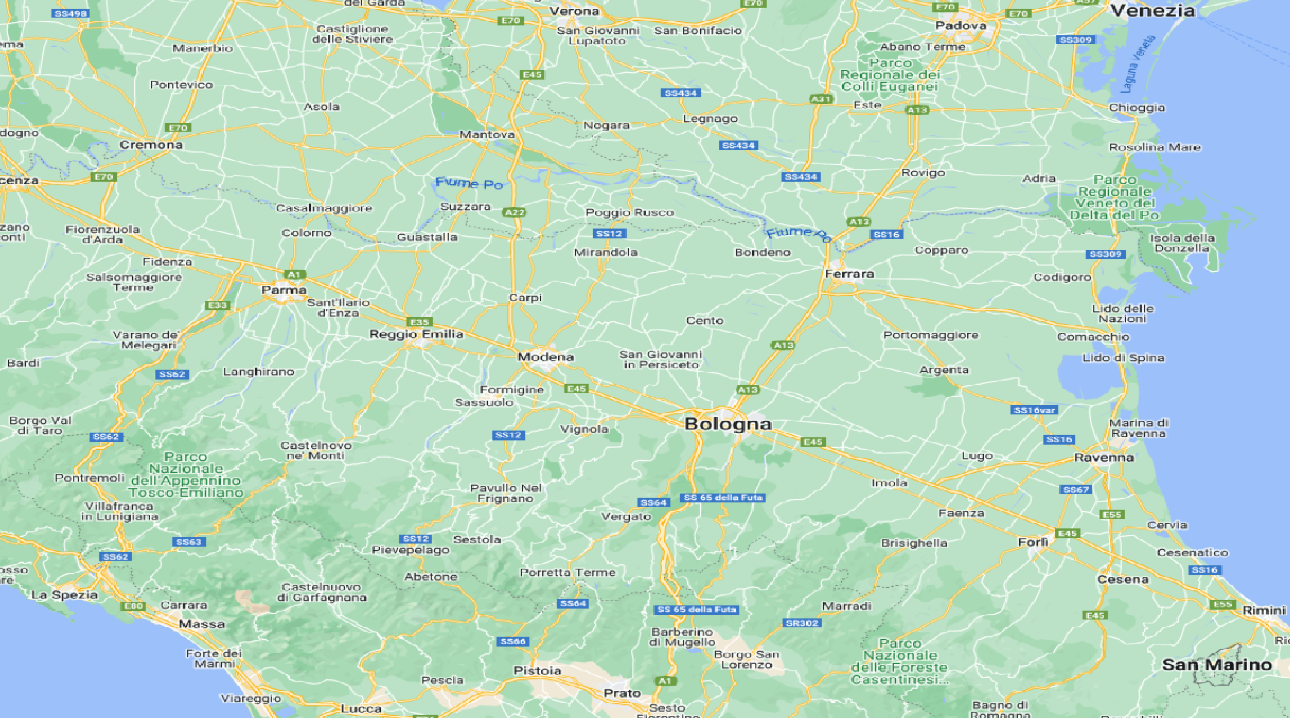
\includegraphics[width=5cm]{images/northitaroads_maps.png} }}%
    \qquad
    \subfloat[\centering Night-time lights]{{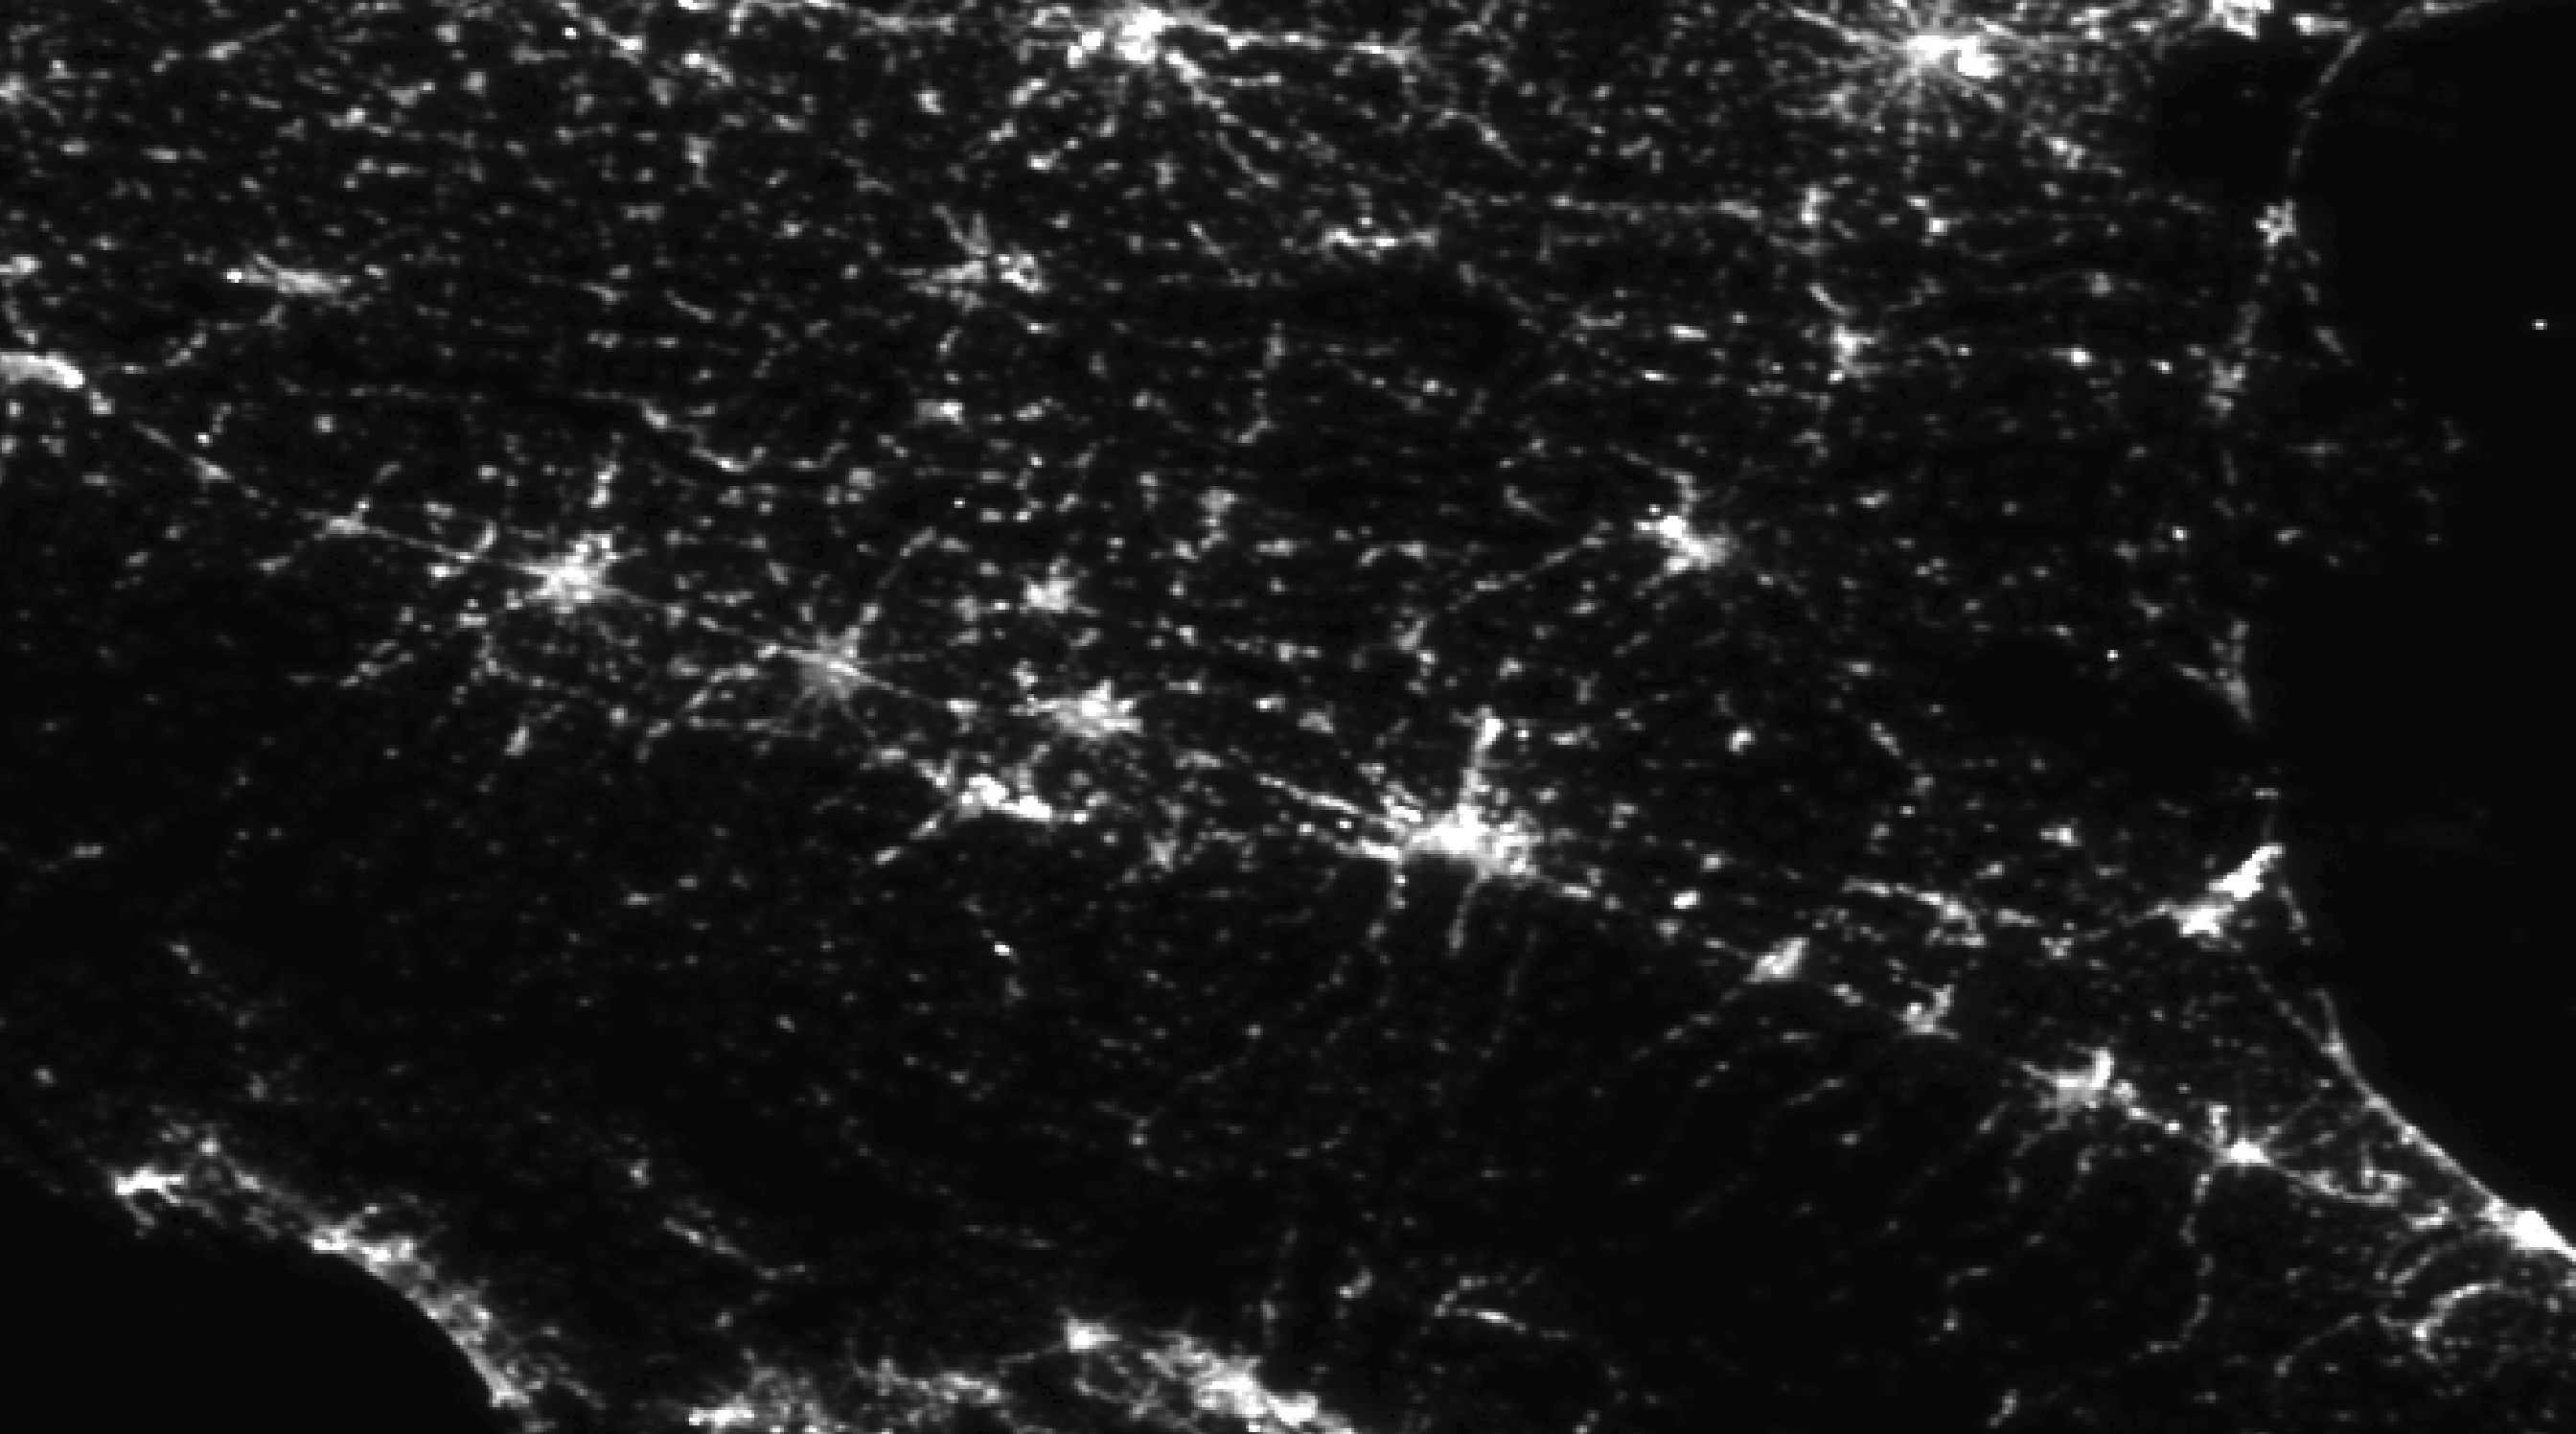
\includegraphics[width=5cm]{images/northitaroads_night.png} }}%
    \caption{North Italy roads - A1 and A14 Highways through Bologna and Modena}%
    \label{fig:northitalyroads}
\end{figure}

\begin{figure}
    \centering
    \subfloat[\centering Google Maps]{{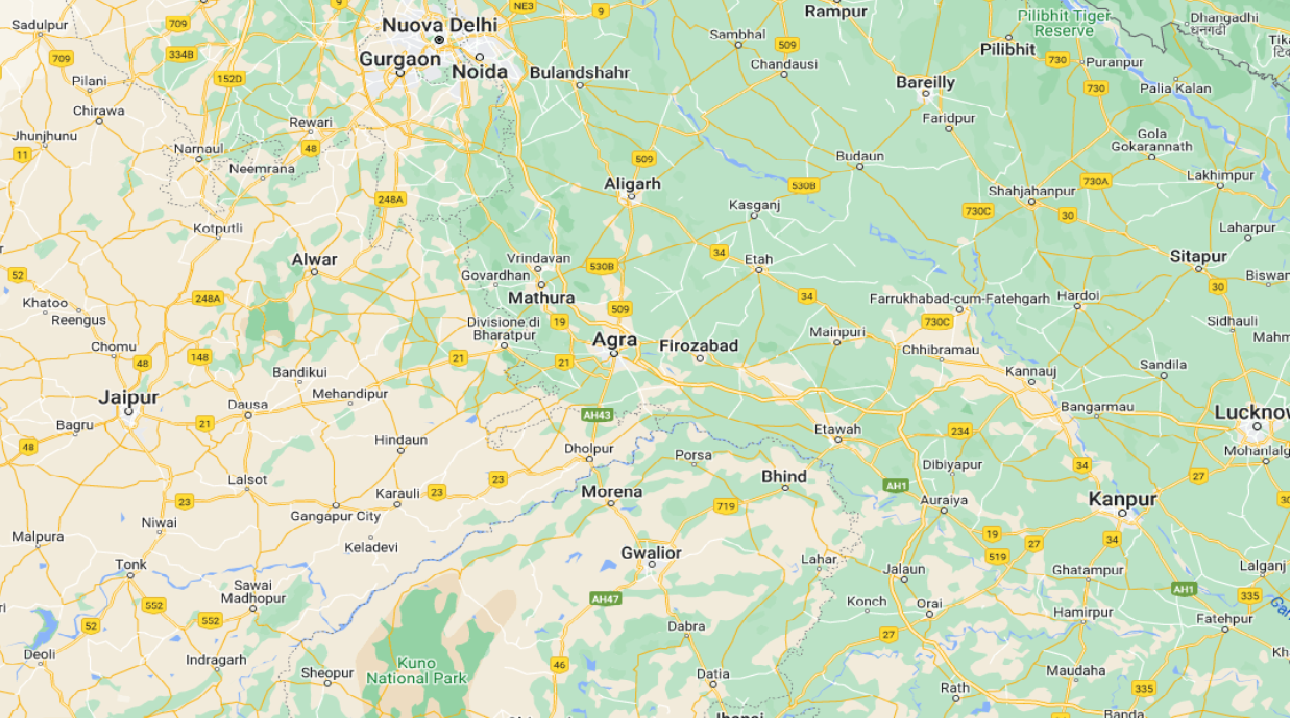
\includegraphics[width=5cm]{images/delhiroads_maps.png} }}%
    \qquad
    \subfloat[\centering Night-time lights]{{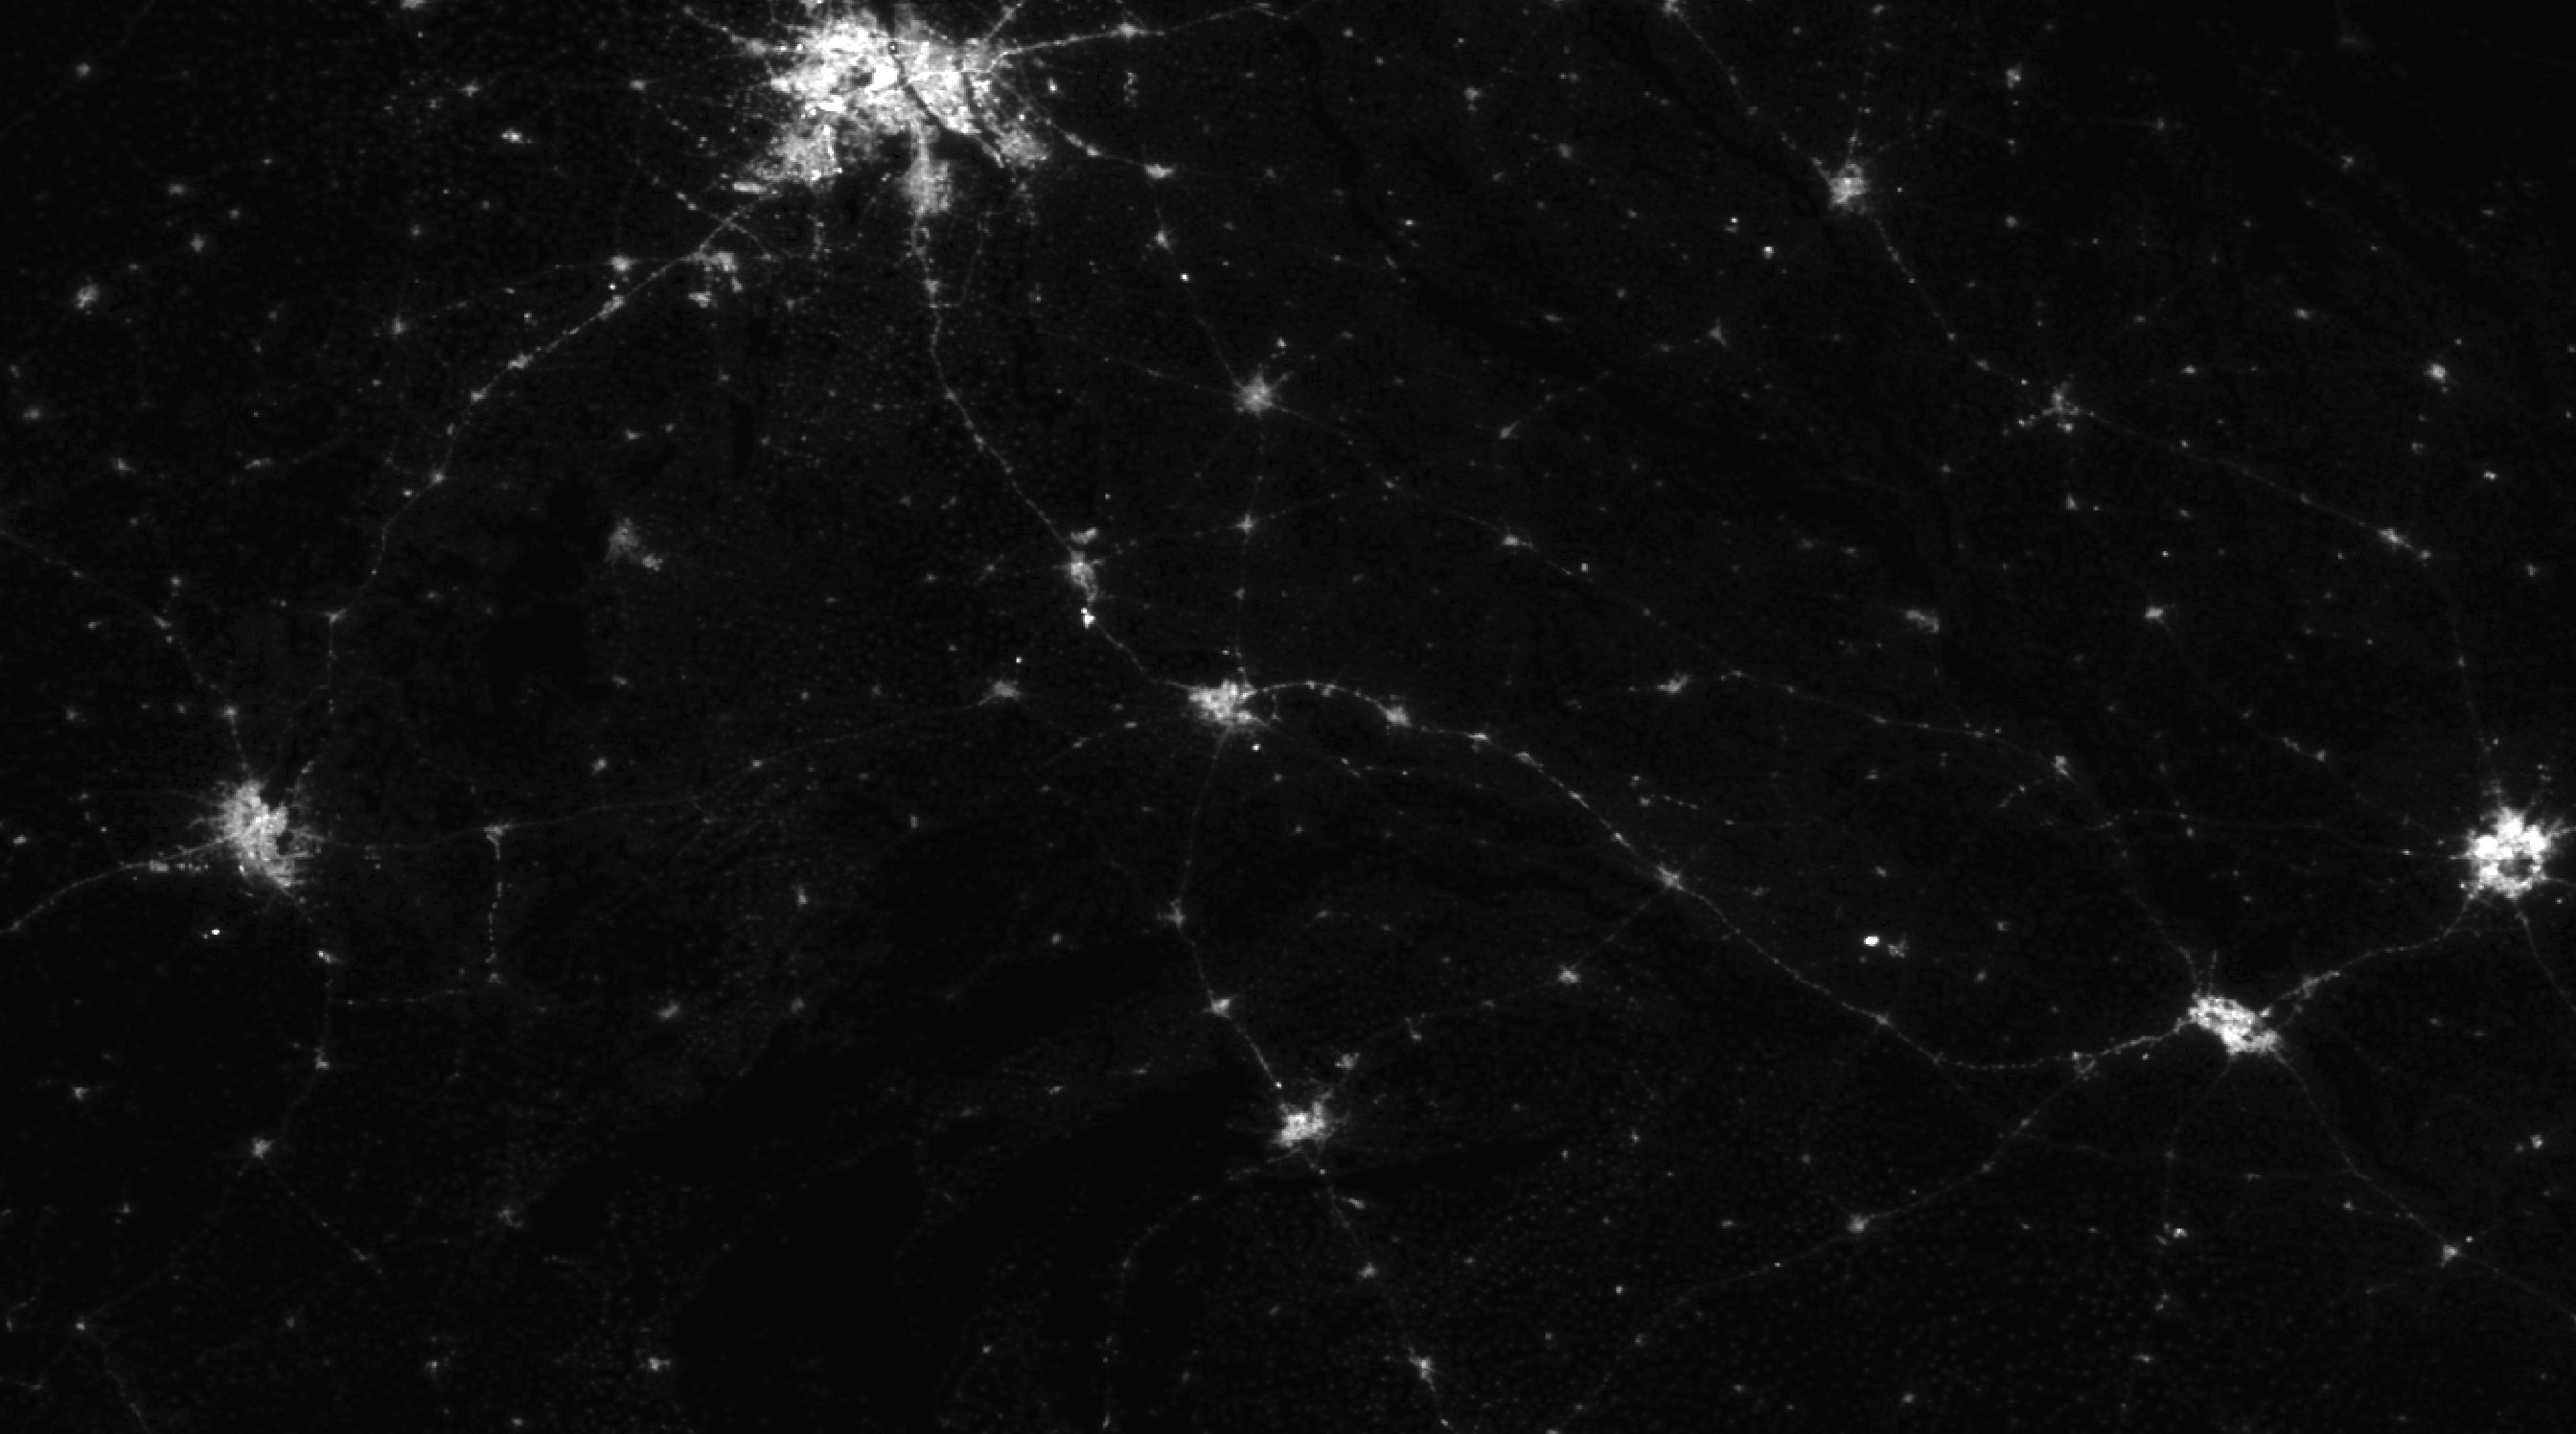
\includegraphics[width=5cm]{images/delhiroads_night.png} }}%
    \caption{New Delhi periphery roads}%
    \label{fig:newdelhiroads}
\end{figure}
Observing night-time lights, the lines of communication between cities or towns can be studied in depth. \autoref{fig:northitalyroads} shows an extract of the main communication line in northern Italy, namely the A1 and A14 motorways connecting the cities of Bologna and Modena with Milan one of the most productive area of the country. \autoref{fig:newdelhiroads}, on the other hand, shows an excerpt of the roads connecting New Delhi in India and peripheral cities.

\subsection{Cities}
Cities are the primary producers of night lights. Studying satellite imagery, the geographical distribution of urban settlements and some of the brightest elements of the cities can be observed, such as major roads,  airports and ports.
Cities night-time lights can be proxy for many economic-related variables. That is population concentration, city dynamism and traffic. It can also be assumed that brighter cities are more economically active and have the resources to mantain such electrical consumption.
\begin{figure}[h!]
    \centering
    \subfloat[\centering Google Maps]{{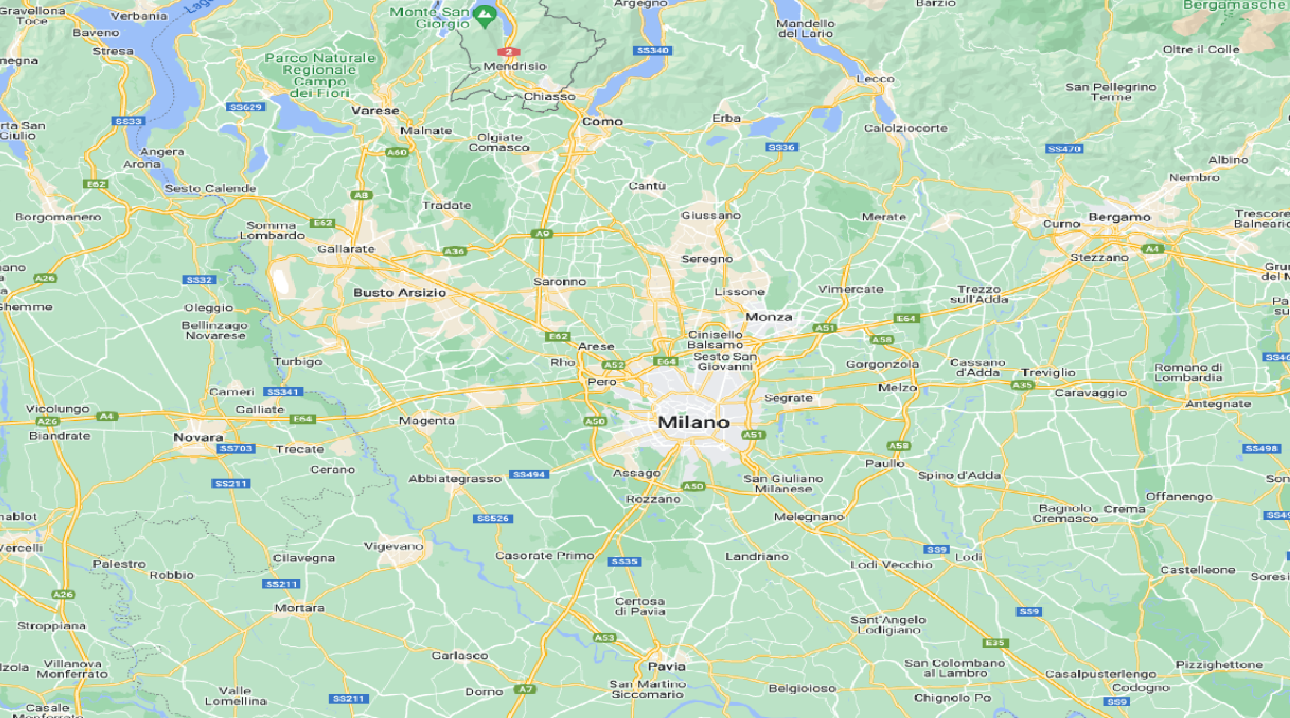
\includegraphics[width=5cm]{images/milan_maps.png} }}%
    \qquad
    \subfloat[\centering Night-time lights]{{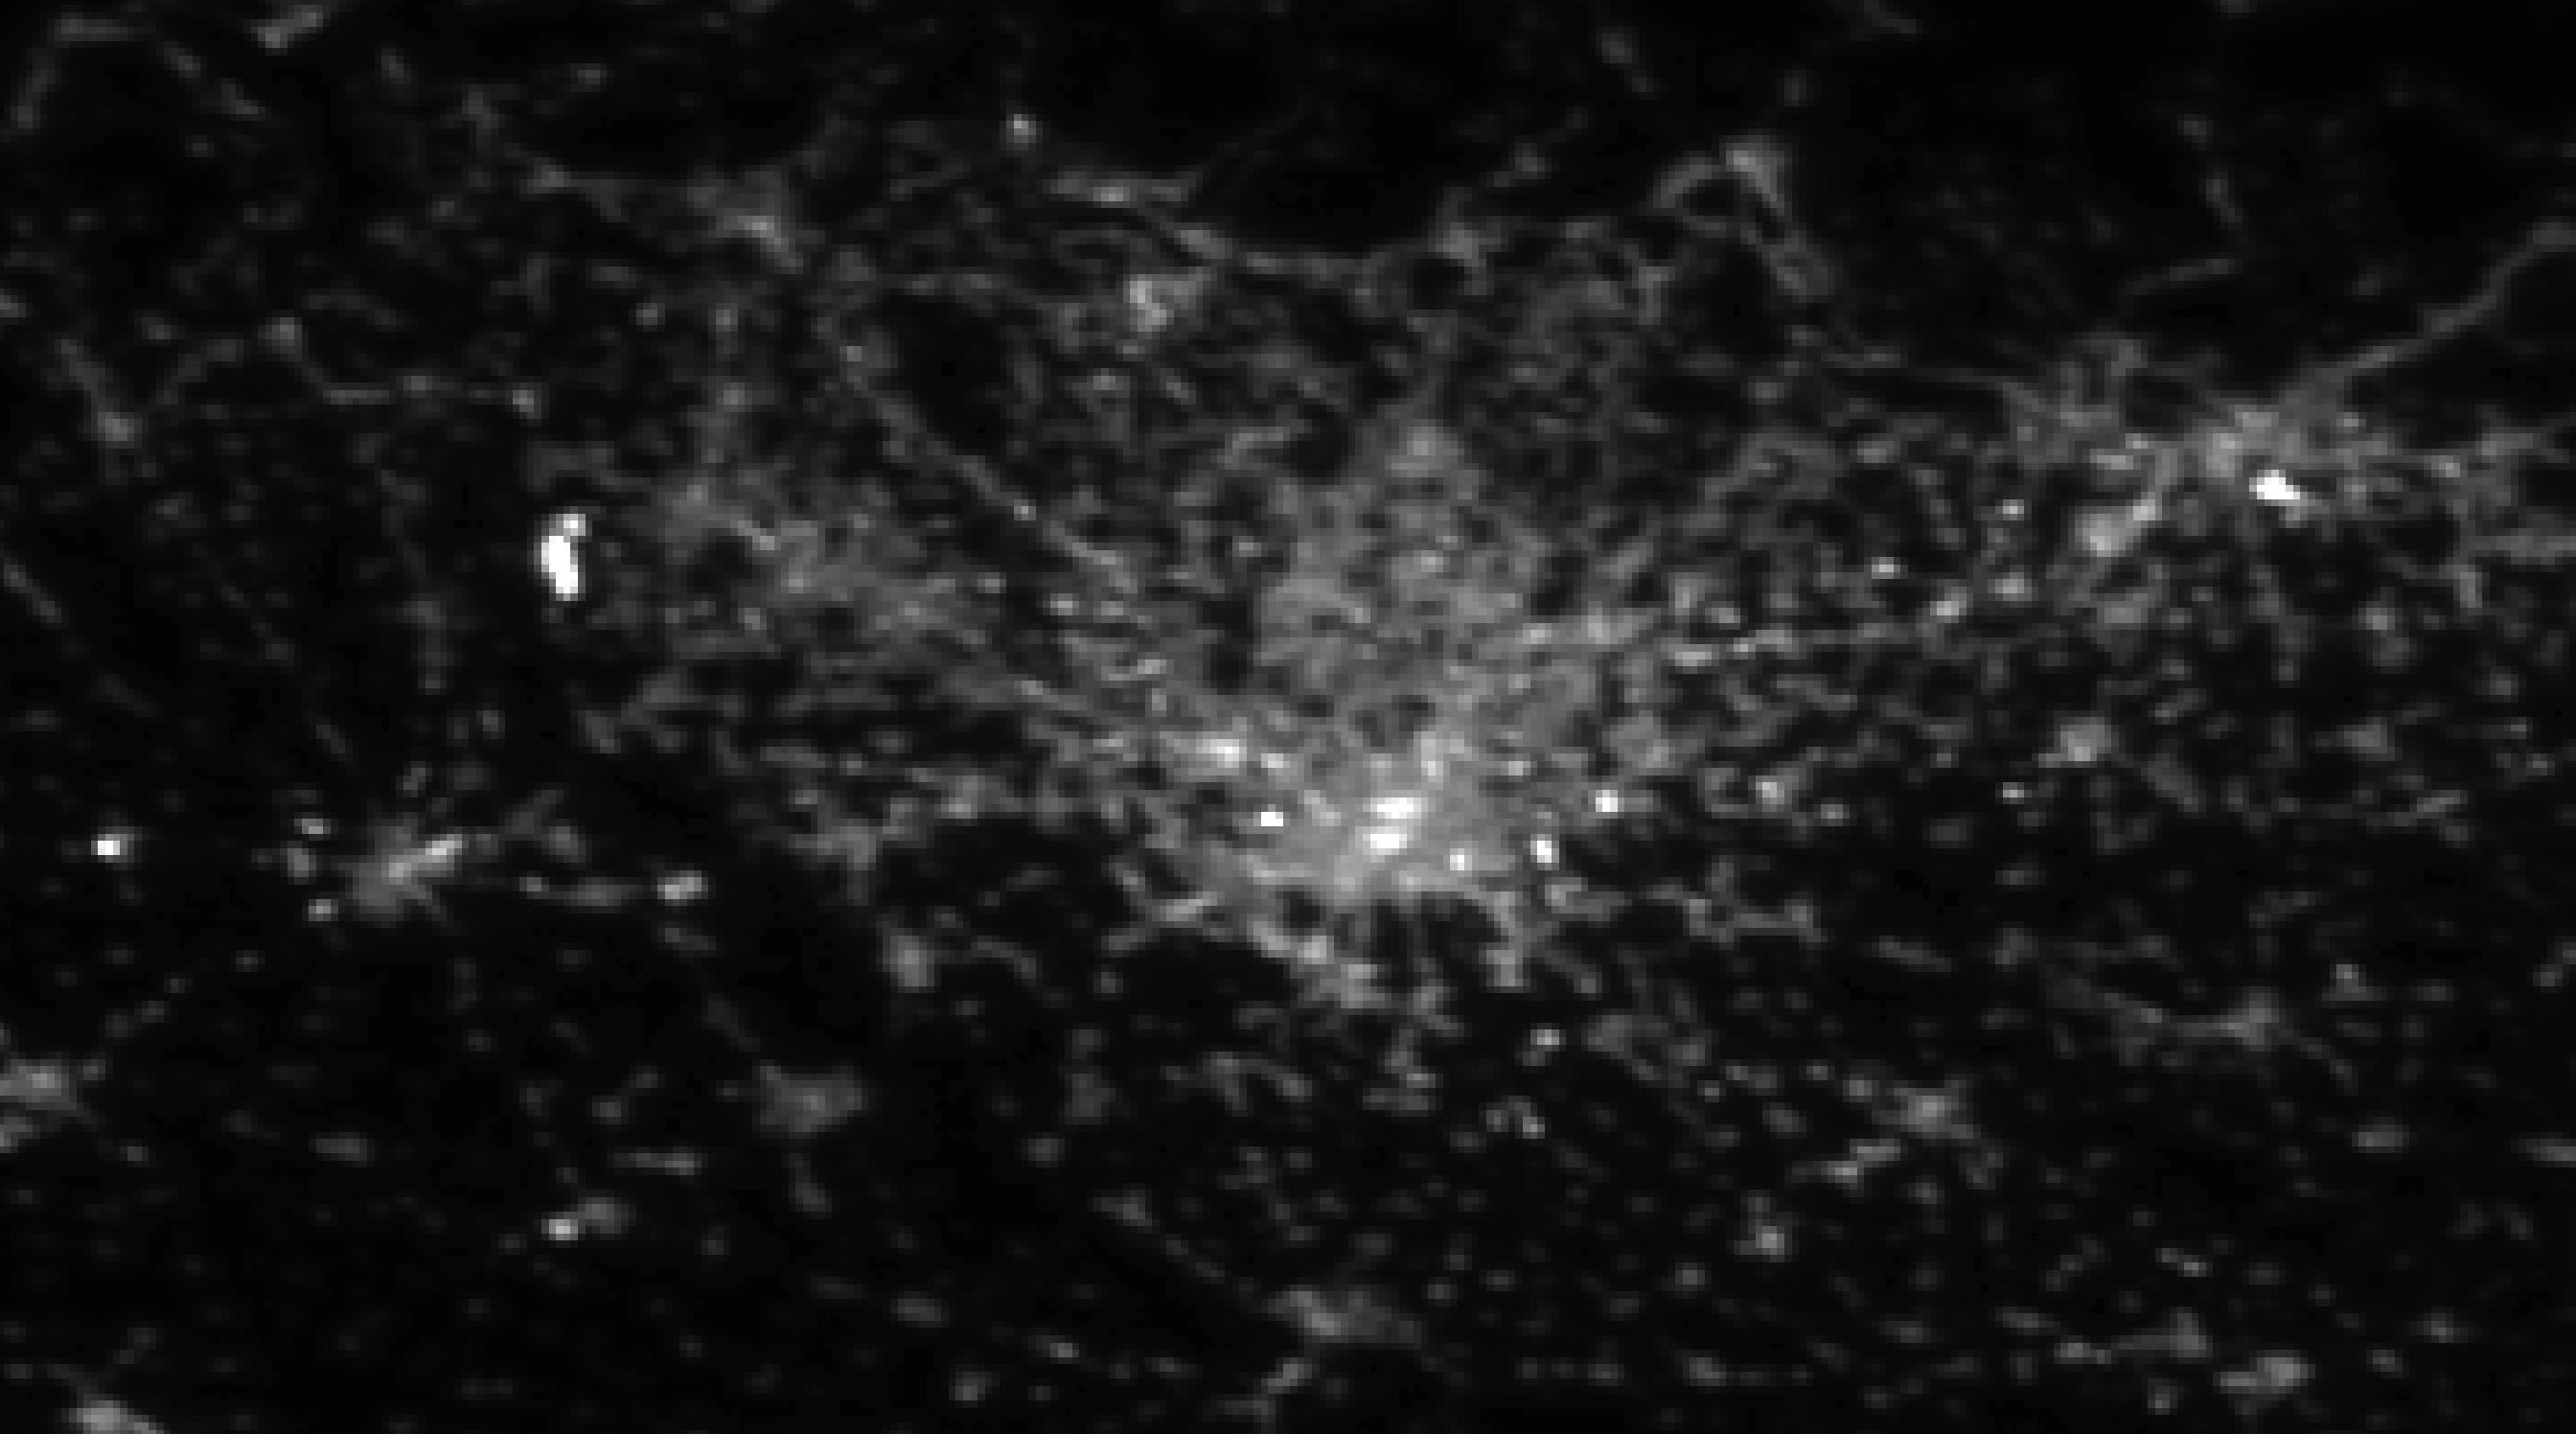
\includegraphics[width=5cm]{images/milan_night.png} }}%
    \caption{Milan - Italy}%
    \label{fig:milan}
\end{figure}
\autoref{fig:milan} shows the city of Milan with \autoref{fig:london} shows London. They are both characterized by well known "web" style. It can be recognized some roads connecting point of interest of the cities and the main airports of both cities can be easily individuated.
\begin{figure}[h!]
    \centering
    \subfloat[\centering Google Maps]{{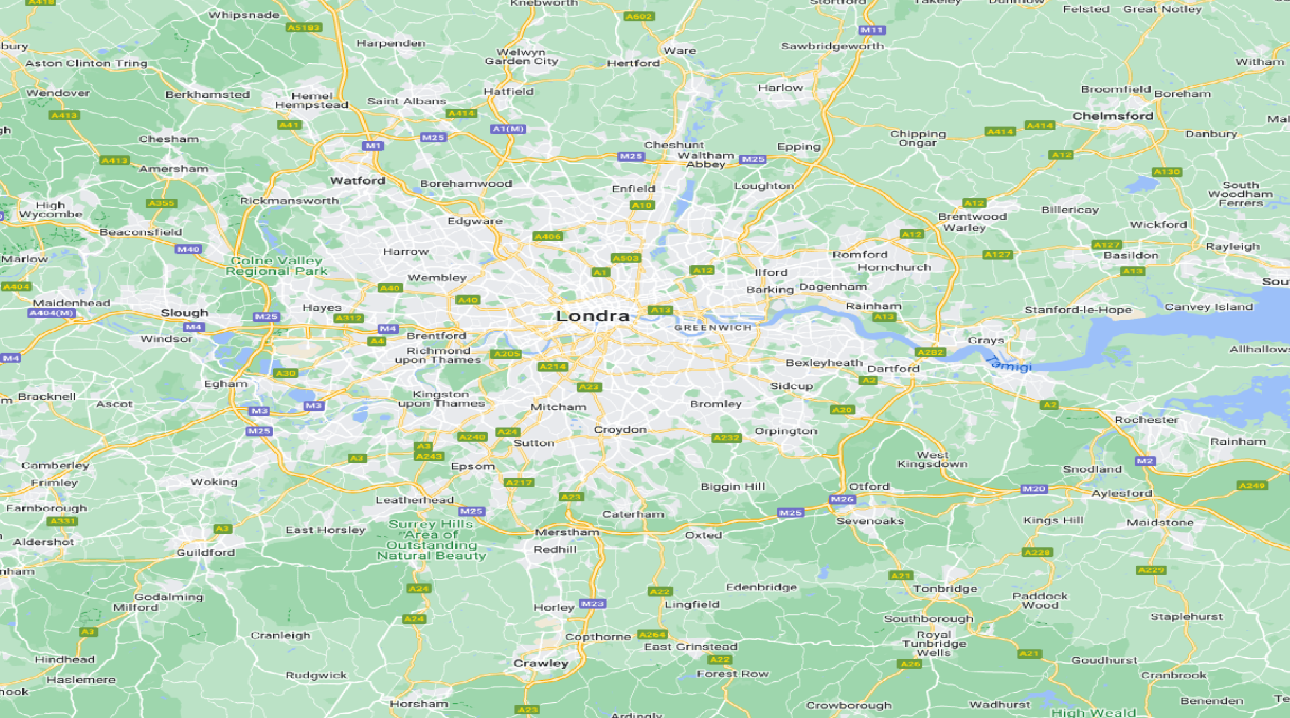
\includegraphics[width=5cm]{images/london_maps.png} }}%
    \qquad
    \subfloat[\centering Night-time lights]{{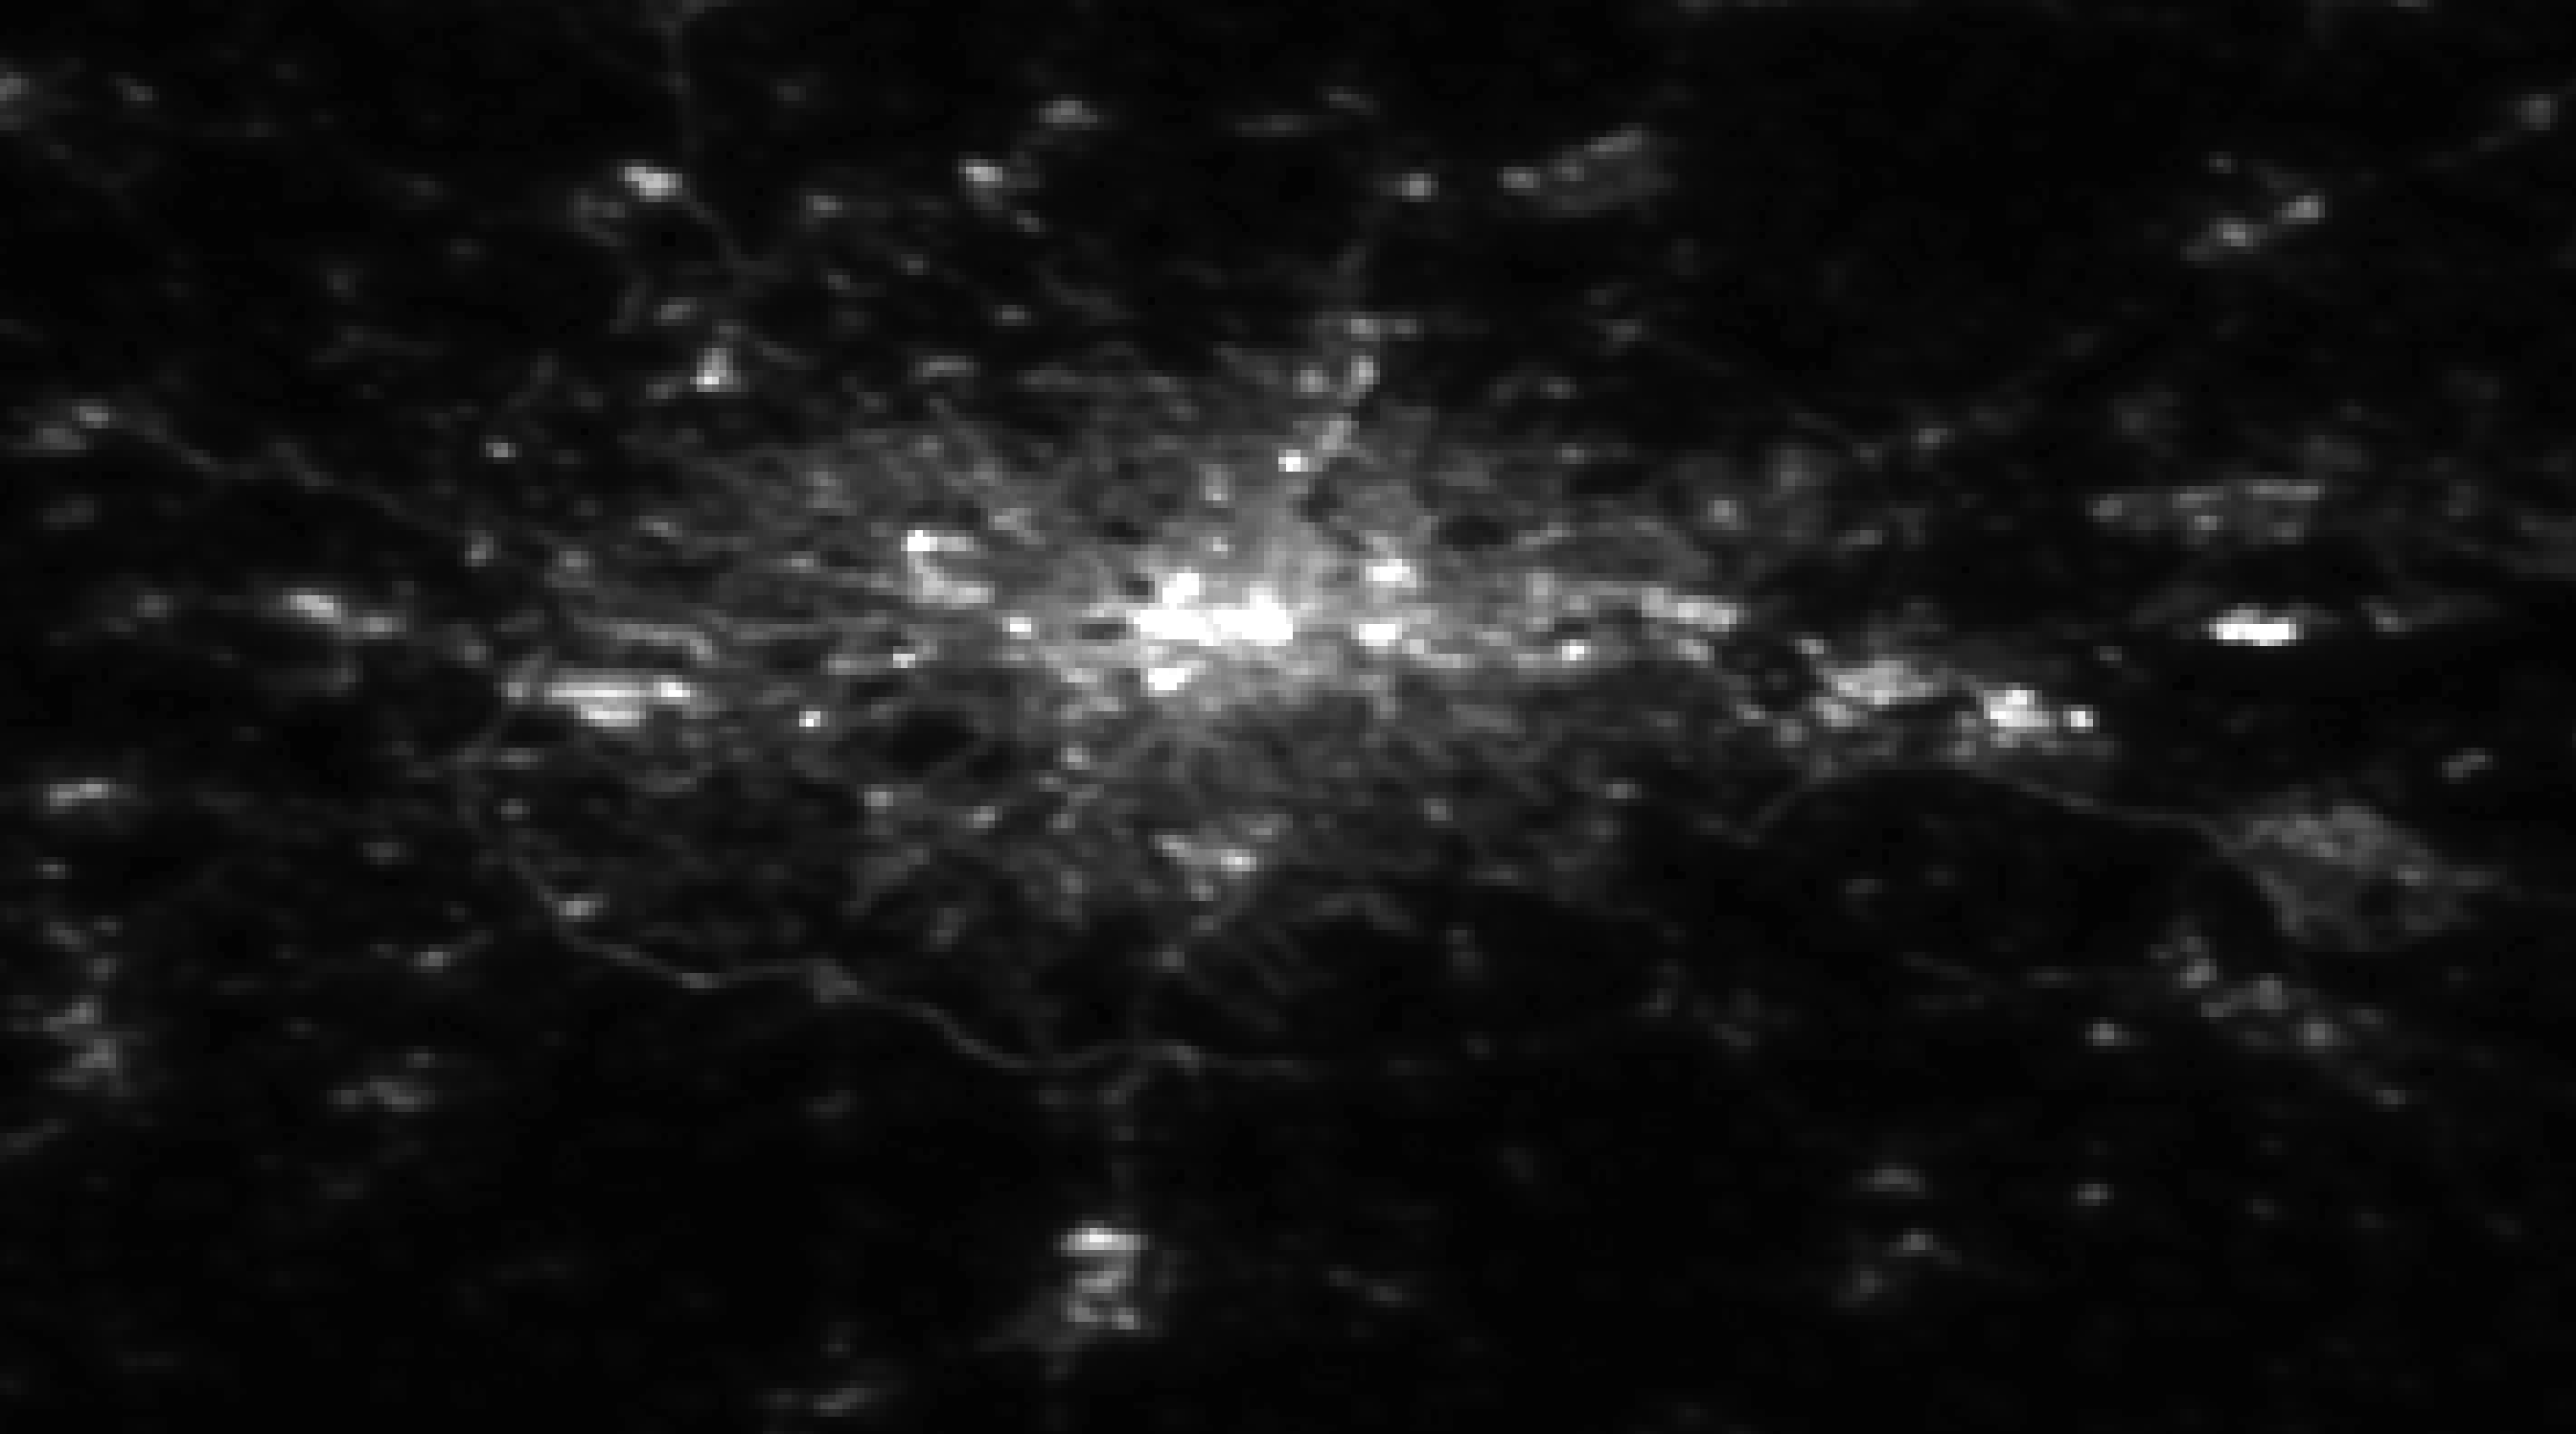
\includegraphics[width=5cm]{images/london_night.png} }}%
    \caption{London - United Kingdom}%
    \label{fig:london}
\end{figure}
\graffito{Note: The content of this chapter is just some dummy text.
It is not a real language.}

\subsection{Airports}
Airports are usually the brightest part of the cities. In \autoref{fig:malpensa} and in \autoref{fig:charlesdegaulle} two of Europe's busiest airports.
\begin{figure}[h!]
    \centering
    \subfloat[\centering Google Maps]{{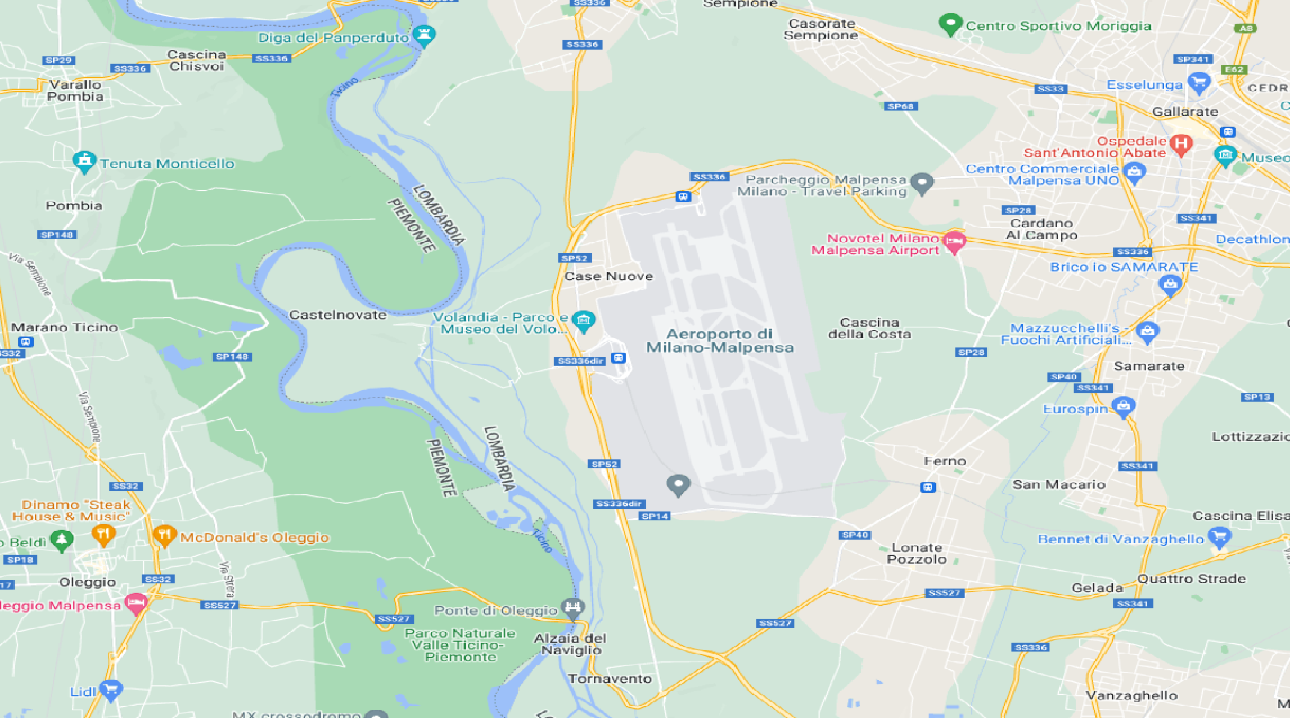
\includegraphics[width=5cm]{images/malpensa_maps.png} }}%
    \qquad
    \subfloat[\centering Night-time lights]{{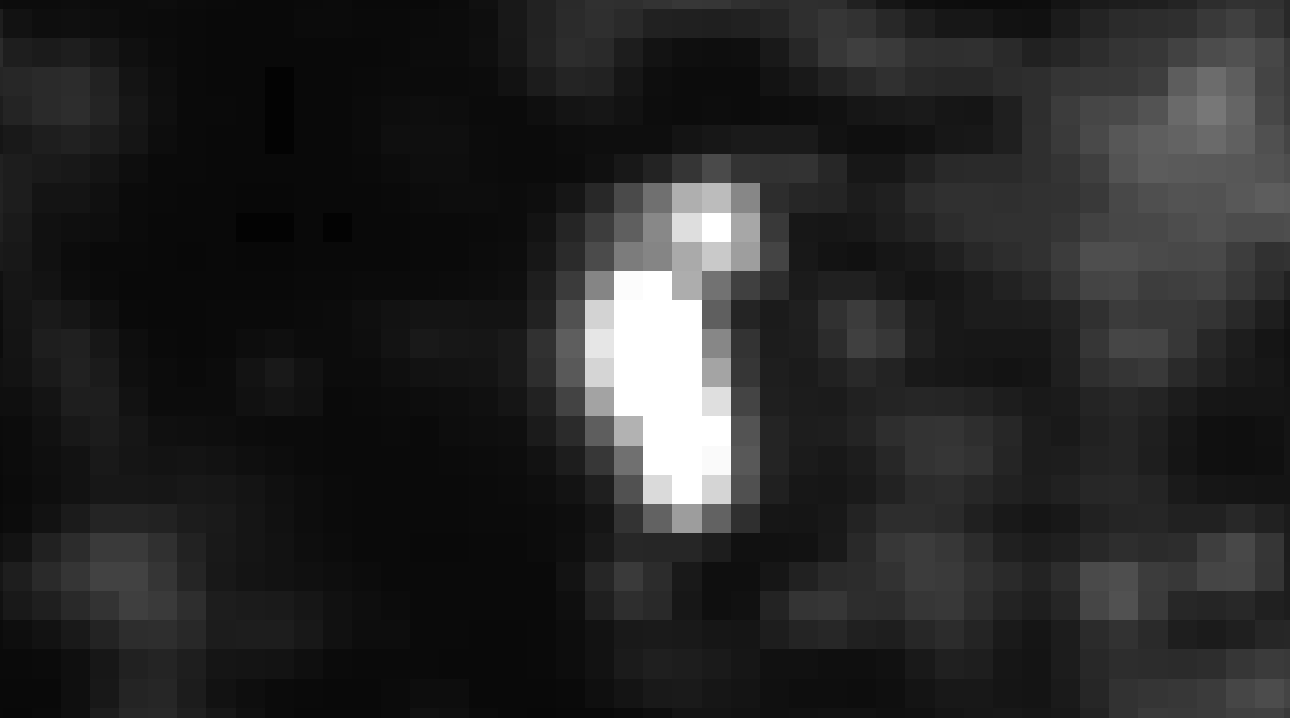
\includegraphics[width=5cm]{images/malpensa_night.png} }}%
    \caption{Malpensa Airport, Milan - Italy}%
    \label{fig:malpensa}
\end{figure}
\begin{figure}[h!]
    \centering
    \subfloat[\centering Google Maps]{{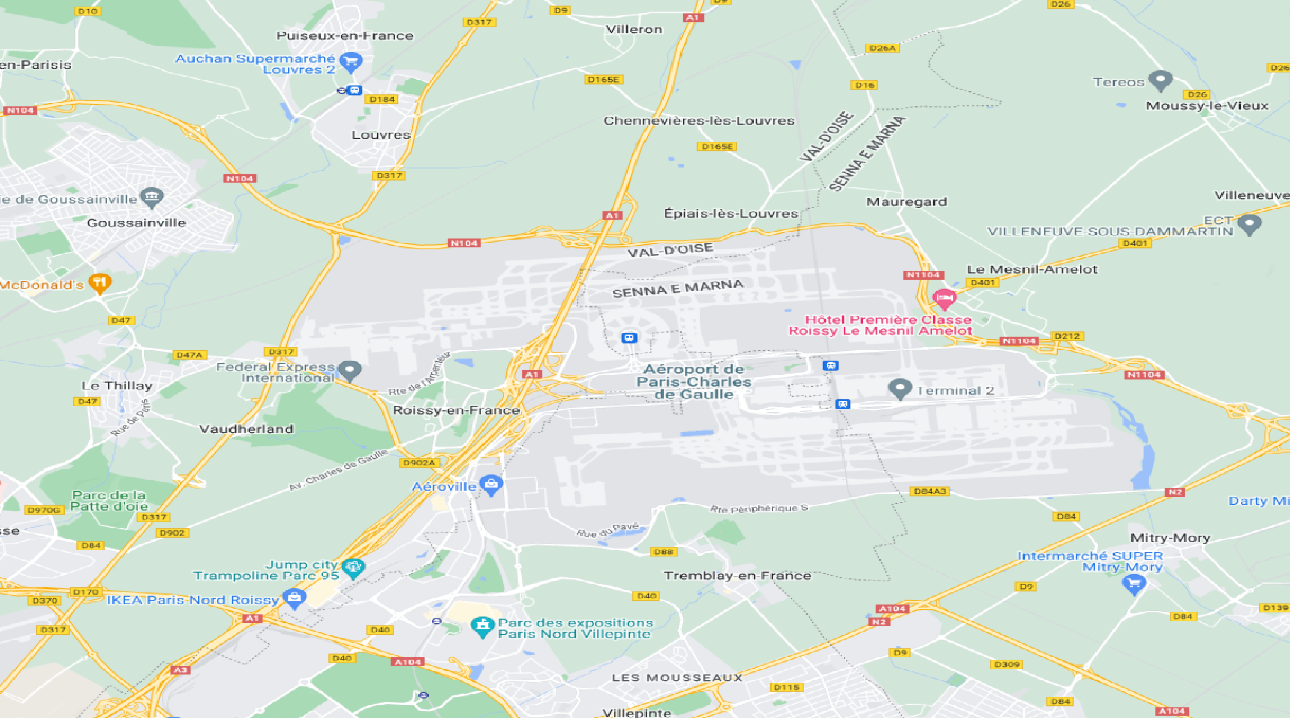
\includegraphics[width=5cm]{images/charlesdegaulle_maps.png} }}%
    \qquad
    \subfloat[\centering Night-time lights]{{
\includegraphics[width=5cm]{images/charlesdegaulle_night.png} }}%
    \caption{Charles De Gaulle Airport, Paris - France}%
    \label{fig:charlesdegaulle}
\end{figure}
\subsection{Ports}
 In \autoref{fig:rotterdam}, the port of Rotterdam. One of the Europe's largest commercial ports. 
\begin{figure}[h!]
    \centering
    \subfloat[\centering Google Maps]{{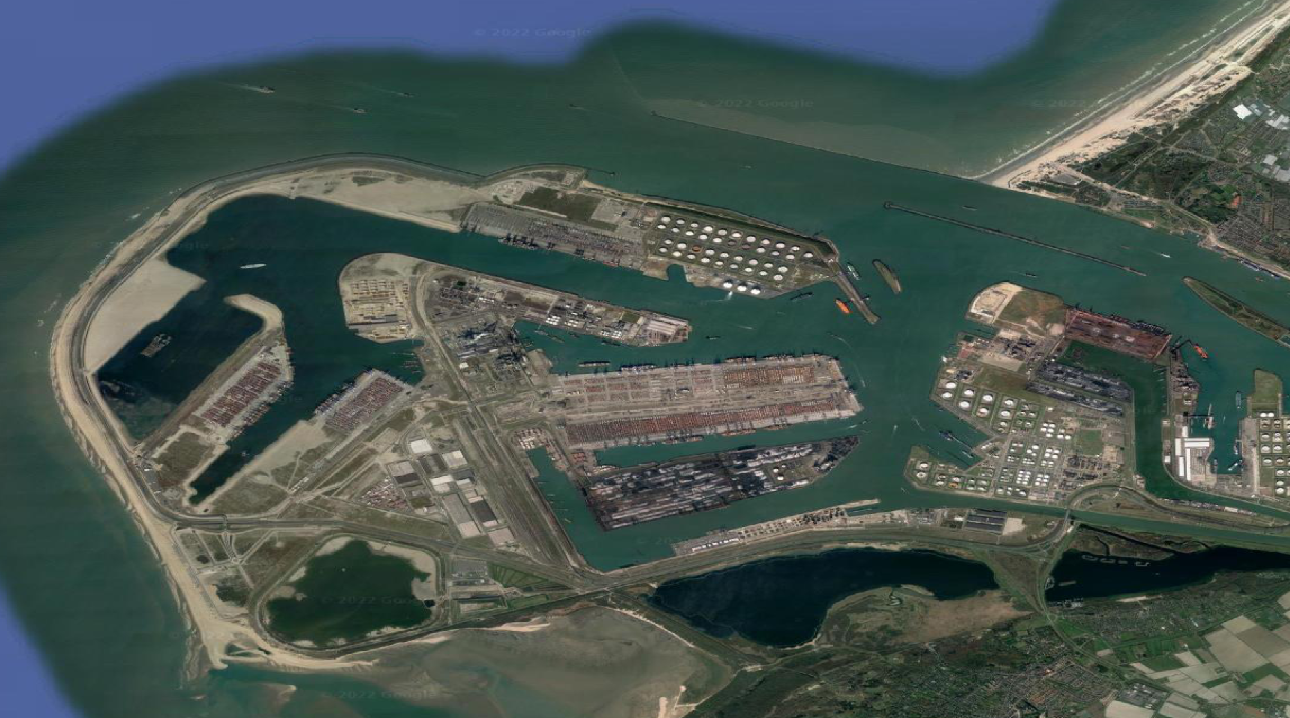
\includegraphics[width=5cm]{images/Rotterdamport_maps.png} }}%
    \qquad
    \subfloat[\centering Night-time lights]{{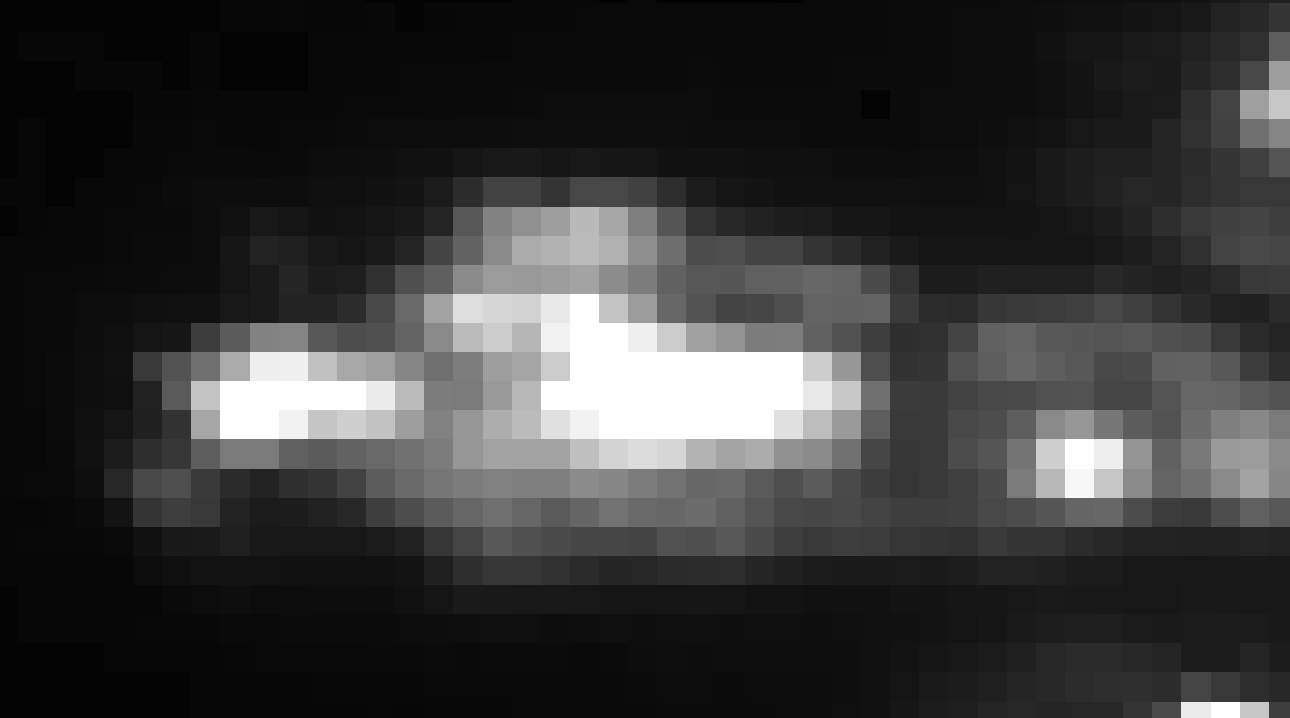
\includegraphics[width=5cm]{images/Rotterdamport_night.png} }}%
    \caption{Rotterdam port - Netherlands}%
    \label{fig:rotterdam}
\end{figure}
\subsection{Human settlements}
 \autoref{fig:nile} shows the night-time image of the Nile. This image is particularly fascinating as it shows a well-known fact in historiography: populations tend to settle around water sources. Indeed, it is unsurprising that most of Egypt's gross domestic product urban settlements are concentrated around its primary water source.
\begin{figure}[h!]
    \centering
    \subfloat[\centering Google Maps]{{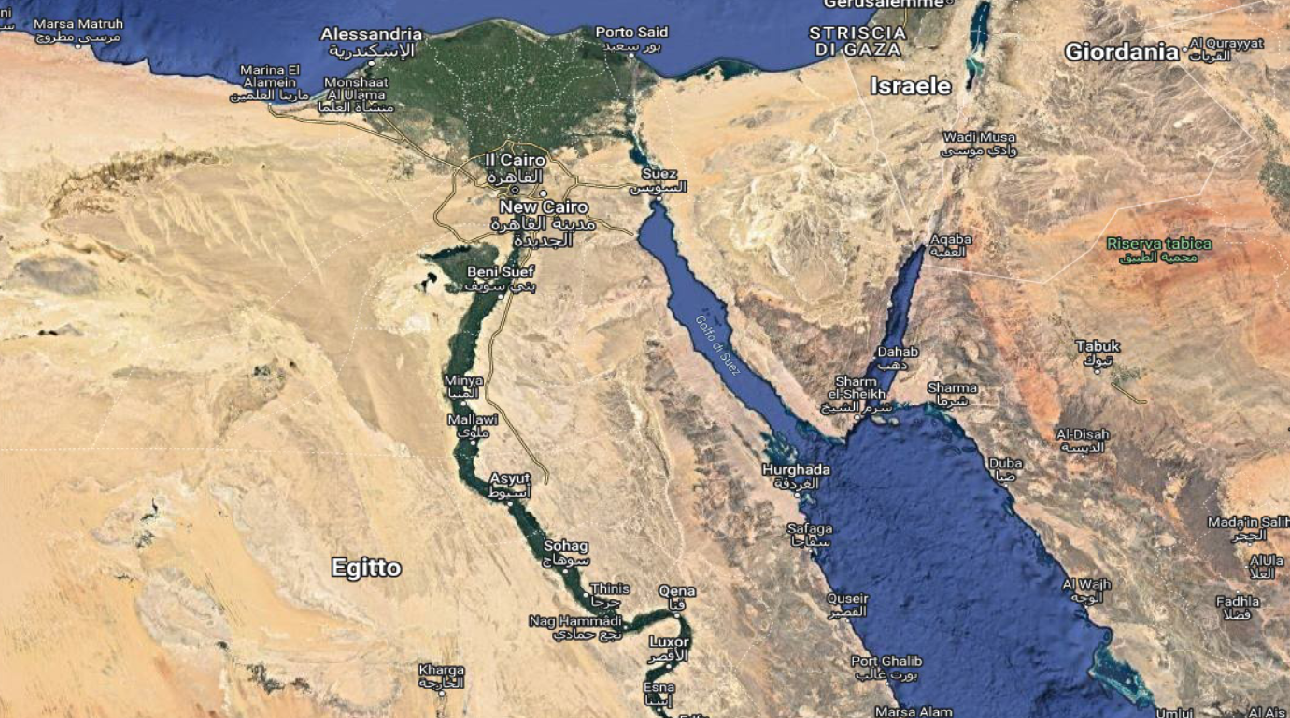
\includegraphics[width=5cm]{images/nile_maps.png} }}%
    \qquad
    \subfloat[\centering Night-time lights]{{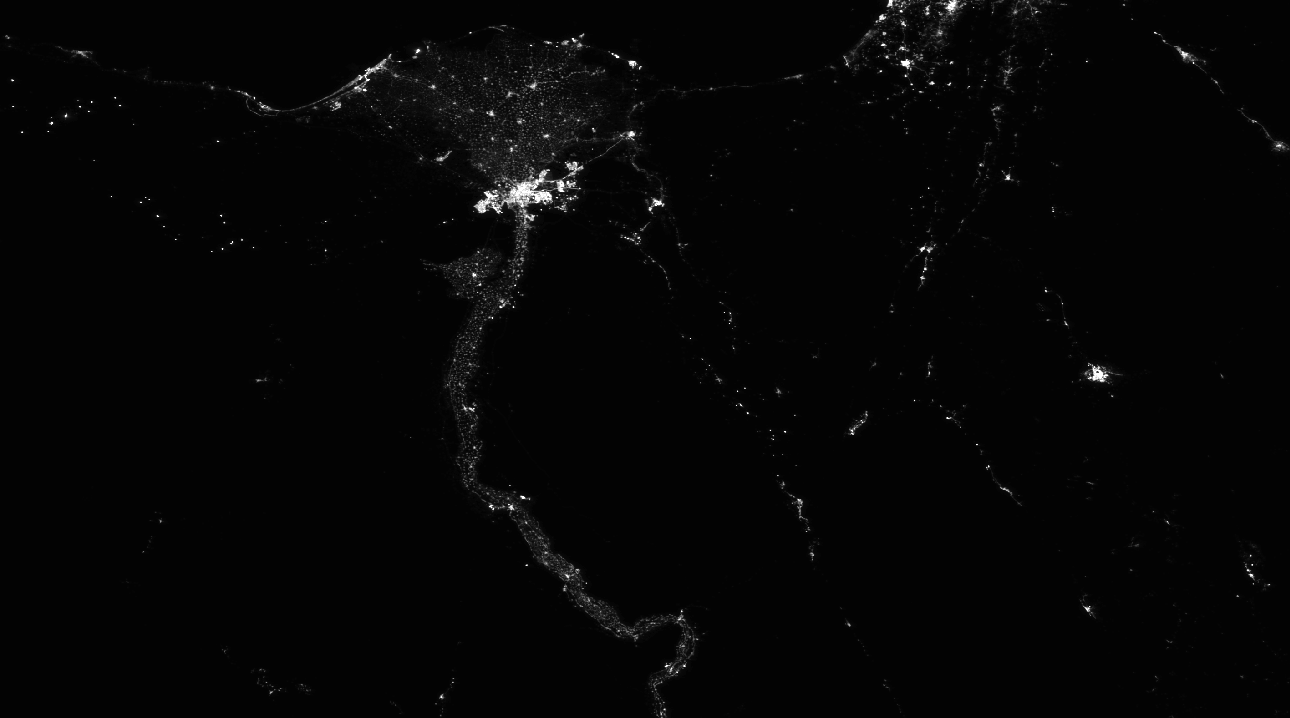
\includegraphics[width=5cm]{images/nile_night.png} }}%
    \caption{Nile river, Egypt}%
    \label{fig:nile}
\end{figure}

\section{Why night-time lights should be adopted} % \ensuremath{\NoCaseChange{\mathbb{ZNR}}}
The employment of night-time lights makes it possible to estimate economic variables under special conditions in situations where we cannot obtain data or have no guarantee of its truthfulness.
Night lights have several interesting properties that have allowed their usage in economic literature. 
\begin{description}
  \item[Exogenous nature:]
 Night-time lights' measurement errors are independent of economic variables \citep{hu2022illuminating}. This allows them to be used as an alternative measure of the economy to the standard ones. In addition, official growth estimates or forecasts pass through government institutes that may have an interest in manipulating data for their political agenda. Night-time lights observable by satellites are much more challenging to manipulate. 
 
In this regard, a popular working paper \citep{martinez2018much}, forthcoming in the Journal of Political Economy in 2022, shows how autocratic states overestimates their growth estimates. Martinez argues that "Since governments themselves usually produce these estimates, they face a recurring temptation to exaggerate just how well the economy is doing".
His results show that the elasticities of night-time lights on GDP are systematically larger in the most authoritarian regimes and that the overestimation averages 35\%.
\item[Worldwide coverage:] night-time lights imagery are captured daily for every area worldwide. This makes it possible to conduct economic estimations in every area of the globe, including countries lacking statistical institutions or areas affected by natural disasters or wars. 

For instance, using data from Project Black Marble, researchers from NASA's Goddard Space Flight Center (GSFC) and the Universities Space Research Association (USRA) analysed the consequences of the Russian invasion of Ukraine on city lights.\footnote{\url{https://earthobservatory.nasa.gov/images/150002/tracking-night-lights-in-ukraine}}
Similarly \citep{li2018night}, studied the dynamics of night-time lights during the Iraqi civil war.
\item[High-frequency data:] data on night-time lights are published every day. As I will show later, for this time-span there are substantial data cleaning problems, however these images lend themselves to daily analysis. Given the long process of estimating official GDP, it can be argued that estimating economic variables through night-time lights leads to high-frequency data. Unfortunately, little has been written about the applicability of economic variables estimated from night-time lights to high-frequency studies. However, also as a result of recent developments in sensor technology (VIIRS), it is possible to consider using these data for policy evaluation analyses.
\item[High-resolution data:]
As I will show in more detail in the following section, the night-time light data is high-resolution data. Namely, we can obtain information for areas of approximately 500m x 500m.
Using these data to study economic variables allows us to reconstruct economic data and allocate information in space. For instance, it is possible to reconstruct geographic maps by calculating the GDP produced in each square kilometre of a country and thus perform zonal statistics in very small areas. With the high-frequency nature of data, it is possible to monitor a restricted area and observe what happens over time or how the economy of the area evolves following the adoption of a certain policy.
\end{description}
%*****************************************
%*****************************************
%*****************************************
%*****************************************
%*****************************************
%\addtocontents{toc}{\protect\clearpage} % <--- just debug stuff, ignore
%************************************************
\chapter{The data}\label{ch:mathtest} % $\mathbb{ZNR}$
%************************************************
Night-time lights data are released by NASA and the EOG project of the Colorado School of Mines. Data is published with different timeframes, i.e. nightly, monthly and yearly.
As I will illustrate in this chapter, the data need to be cleaned before being used, and the two sources use different data cleaning algorithms; NASA has a faster publishing rate. New data is released each night just over an hour after the satellite took the imagery. On the other hand, the EOG data, from the analysis I have carried out, implements a more effective data cleaning algorithm. Moreover, NASA files are published in tiles, small portions of space that must be processed before they can be used. Each tile must be geolocalised in space according to the order in which the tile is positioned.

\section{Dealing with satellite data}

Night-Time light data are distributed in georeferenced \textit{.tif} images, which are images that contain map projection information, namely the coordinate reference system. 
\textit{Raster} files are  $n \times k$  matrices that divide the observation surface into rectangular pixels.

\begin{figure}[h]
    \begin{center}
    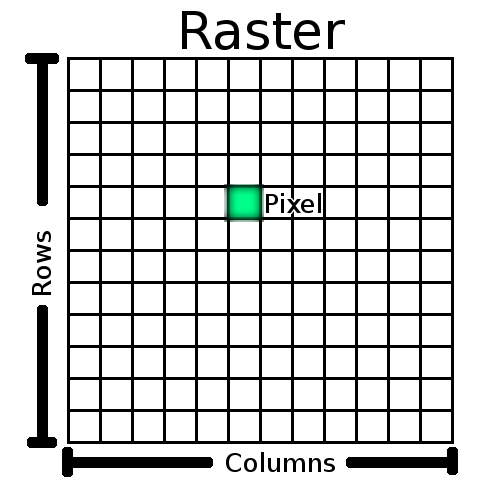
\includegraphics[width=7cm]{images/raster_dataset.png}
    \end{center}
    \caption{Raster representation - Source: Qgis Documentation.}
\end{figure}


With night-time lights, each cell of the raster matrix contains the reflectance measured in that specific portion of the globe.
Depending on the sensor's technology mounted on the satellite, the pixels will capture smaller portions of the globe, producing higher resolution images. 

Given the circular motion of the satellite orbit, the resolution is measured in \textit{arc/seconds}. Regarding the two main technologies in the night-time lights industry, the VIIRS sensor data has a resolution of 15 arc/seconds (circa 500 metres at the equator), while the previous DMSP sensor data is about 30 arc/seconds (circa 1000 metres at the equator). 
\begin{figure}[h]
    \begin{center}
    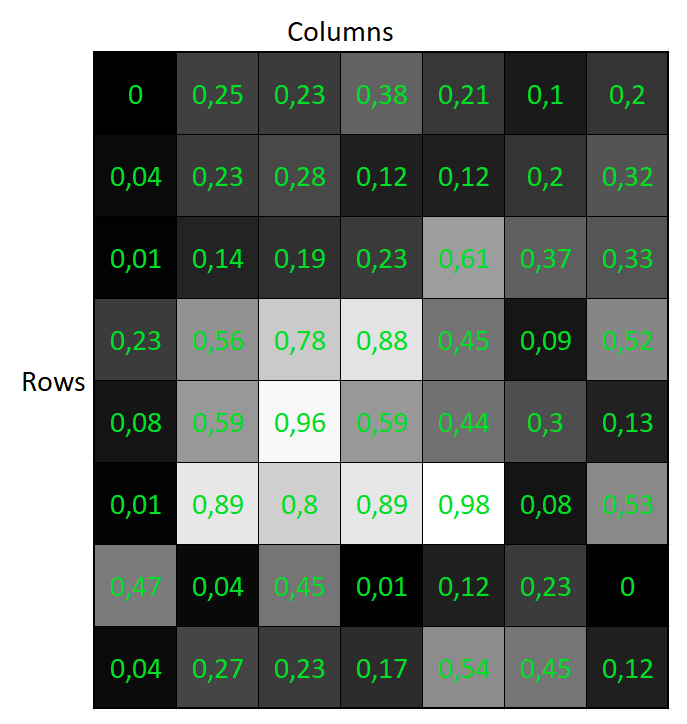
\includegraphics[width=7cm]{images/raster_night.png}
    \end{center}
    \caption{Night-time raster representation.}
\end{figure}
The geographic reference system divides the Earth into 360 equal segments called degrees. Each degree contains 60 minutes and, therefore, 3600 seconds.
An arc-second is the geographical distance measured on the surface of the Earth after one second's rotation, or 1/3600th of a degree.
At the equator, one arc/second of latitude corresponds in metres to one arc/second of longitude. However, the further one moves towards the poles, the equivalent of one arc/second in longitude decreases while latitude remains stable.
  
To perform \textit{zonal statistics}, i.e. statistics of delimited areas of the globe, it is necessary to delimit the raster files with another file that contains georeferenced information about geographical boundaries. For this purpose, most of the time, \textit{Shapefiles} or \textit{GeoJson} are used, which are called "polygon files". These files contain information about the boundaries of the geographical regions to be studied. As with raster files, polygon files can also have different resolutions. In this thesis, I will use the data with the highest possible resolution distributed by GADM.
\begin{figure}[h]
    \begin{center}
    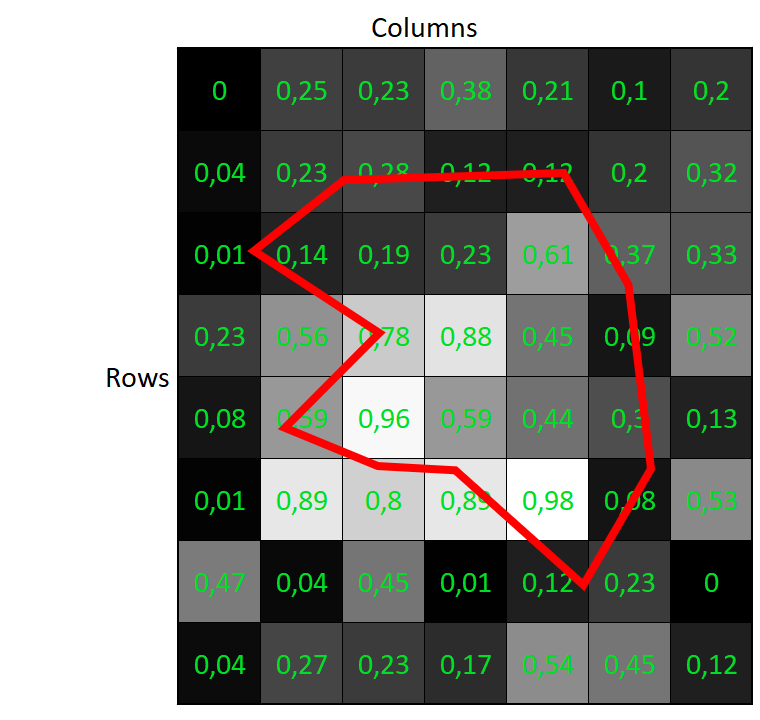
\includegraphics[width=7cm]{images/raster_night_cover.png}
    \end{center}
    \caption{Night-time lights extraction process representation.}
    \label{fig:extraction}
\end{figure}
GADM is a free open-access database of global administrative areas that publishes high-quality border data.
The geographical area to be studied is obtained from the intersection of the raster file and the polygon file such that a statistical function can be applied. For this thesis, I will make use of summation, but spatial variance can be used as well.
Given a $m\times n$ raster file, the summation is defined as:
\begin{equation}
    TotNTL=\sum_{i=1}^n\sum_{j=1}^m x_{ij}.
\end{equation}
An important consideration must be made regarding the data extraction process. It is legitimate to ask how to deal with pixel values only partially contained within the geographical boundaries of interest as in \autoref{fig:extraction}. In this thesis, I will use the R package {\it exactextractr}, which is the most refined package for data extraction. This package, unlike {\it raster} and {\it terra} alternatives, extracts values by weighting them for effective coverage. 
A final note on the analysed data is the weight they occupy on the disk. An annual panel analysis of 11 years results in a data volume of around 120 gigabytes multiplied by 12 (i.e. around 1.5 terabytes) if the analysis is carried out with monthly data. This results into long analysis processes and so high computing power is needed.

\section{Data problems}
Managing satellite data is complex. One of the difficulties is dealing with some capturing issues that, without correction, may give biased data. For this reason, research on the best algorithms for cleaning and producing data does not stop, and new types of algorithms are constantly updated. The three main problems we face are:
\begin{enumerate}
\item \textbf{Cloud Coverage:} As argued earlier, one of the many purposes of night-time lights was to study the presence of clouds. It is, therefore, not surprising that, if only interested in the dynamics of the emitted night-time illumination, the complete or partial overlay of clouds may result in missing or dirty data. 
The data published by both NASA and EOG also include detailed information on the areas where clouds were present at the time of the capture. It is up to the researcher to choose whether the amount of daily data without cloud cover is sufficient for her purposes. 
A possible solution is to use the information on the areas covered by clouds from other periods. To do this, the time window of analysis must be increased. Several algorithms have been developed to aggregate daily data into monthly or annual surveys. 
The operation is not complex and works as follows, given several daily surveys in one layer of raster information and another layer with the different cloud cover of the respective days, the algorithm takes only the values of the non-covered or partially covered areas and through a statistical function (mean or median most of the time) reconstructs a complete image.
Although very rare, a particular area may be covered for a whole month by clouds that prevent a correct representation of the actual light emitted. For this reason, it is necessary to consider the percentage of cloud-free observations of that month. Otherwise, data would be biased and annual aggregates may have to be used.
\item \textbf{Natural lights:} when measuring night-time lights, the presence of natural lights is a problem. Natural lights include sunlight, moonlight, reflections, burning biomass and other ephemeral events.
Dealing with these problems is much more complex than with cloud coverage. Different strategies have been adopted.
The most common of the strategies is cleaning through data aggregation, as seen above. This is because some of these natural lights have a seasonal nature. For instance, some areas of Northern Europe in the summer months suffer from overexposure to light at night, and the resulting images have entire areas burnt out. This kind of problem can be solved satisfactorily by aggregating an entire year's daily images.
On the other hand, other natural light sources have no seasonal character, namely, among the others, burning biomass and reflections. In this case, the remote sensing literature has treated these problems as outliers and proposed some solutions. For instance, the first version of EOG data used a histogram-based technique in which the tails were cut off. This data was further cleaned by eliminating background noise by identifying a minimum threshold in the neighbourhood of each pixel.
\item \textbf{Stray Lights:} In optics, stray lights are defined as instrumental noise in optical systems due to unwanted light, namely reflections or lens imperfections. Again, various algorithms have been created to deal with this issue. EOG publishes two types of data, "vcm" is the raw non-stray light corrected data, while "vcmsl" is the cleaned data.
\end{enumerate}
The data I will use in this thesis are those of the EOG project. In the last years, they adopted three versions of the cleaning algorithm, V1.0, V2.0, and V2.1, which have gradually become more and more sophisticated in handling the issues mentioned above.
Version 2.0 of the algorithm updates the threshold detection used to eliminate the light background in a sophisticated manner. Without intending to be exhaustive, the new algorithm calculates the median of the maximum values of the multiyear time series, weighted for cloud-free observations. A scattergram of the observations is then created by plotting the percentage of cloud free versus the data range, and a gamma curve was fit to lie above the scattergram noise levels. Gamma curves are usually adopted in optics applications. In this case, the gamma curve sets a threshold for each globe observation for each cloud-coverage level. 
\begin{figure}[h!]
    \centering
    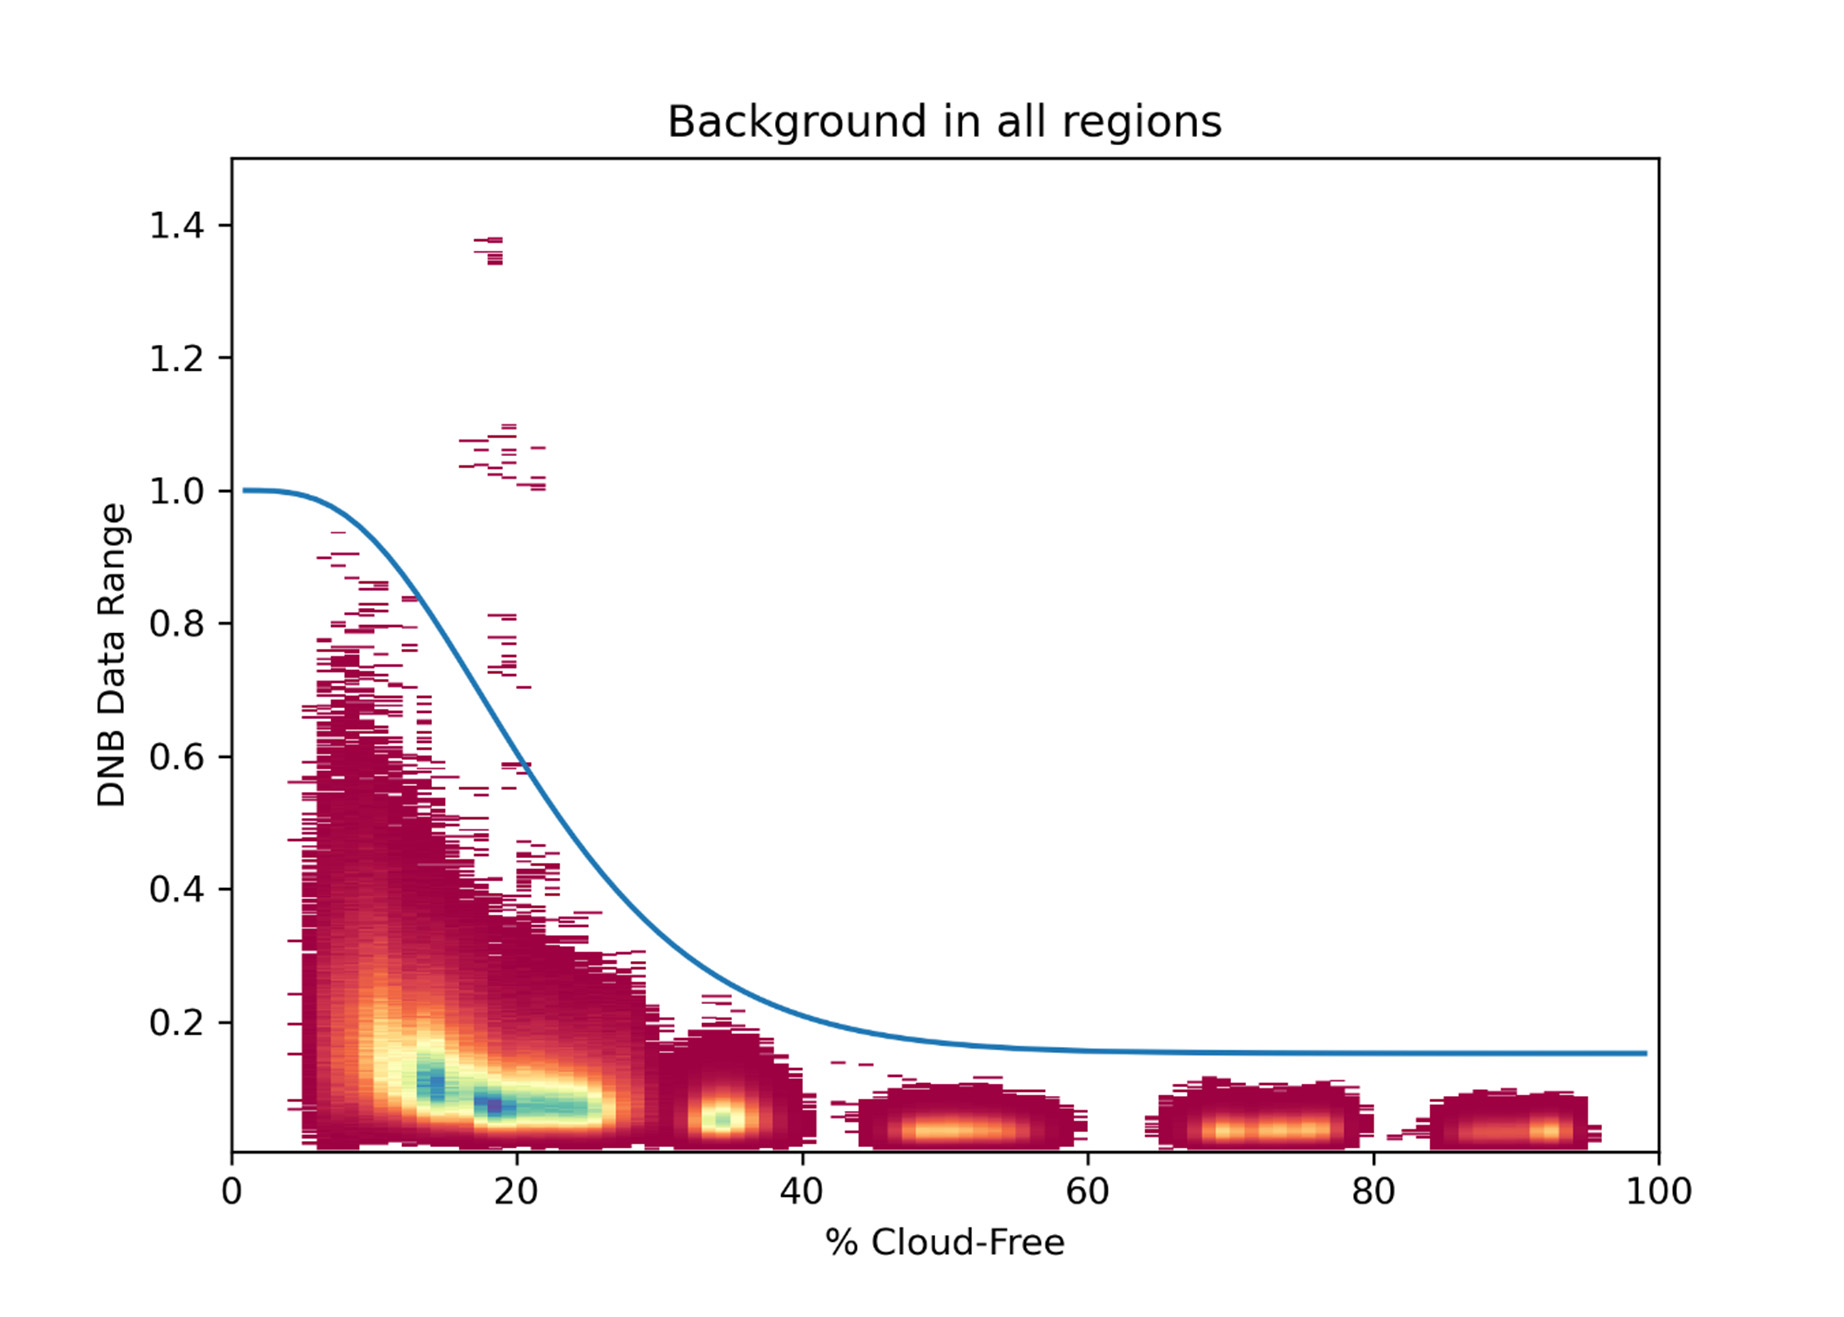
\includegraphics[width=13cm]{images/scattergram.jpg}
    \centering
    \caption{Scattergram and gamma curve - \citep{elvidge2021annual}.}
    \label{fig:scattergram}
\end{figure}

Finally, much noise was caused by the Aurora Borealis. Increasing the threshold too much would have resulted in a significant loss of information in other areas of the globe. Therefore, a \textit{manual} approach was adopted by overlaying a layer on the residual noise in the north and south aurora zones.
As mentioned earlier, although these algorithms \citep{elvidge2021annual} constitute state-of-the-art in the field, they do not correct for some peculiar events. When analysing the data, I found some anomalies. If I extract the maximum observable values, I find very high values in Russia in the middle of nature partly caused by gas flaring, a phenomenon due to the high quantity of natural gas processing plants in the region.
This phenomenon is particularly relevant for the purpose of this thesis because it causes huge light concentrations that leads to pixels 200 times brighter than the most populated capitals in the world. 
These points are few, but they take high values, and the sum extraction process leads to very different results in some countries. In the following sections, I will try to deal with this problem.
Finally, after analysing the data, I found that between 2016 and 2017 there is a big jump in the levels of night-time lights for many countries in the world. The reason seems to be that as of 12 January 2017, the EOG team changed the methodology for converting the raw data to radiance data.
Specifically, the dark offset term used in converting the raw counts to radiance was changed from a dark ocean view to a space view, resulting in a slight upward radiance shift per each data point. This was first documented by \citet{elvidge2020indicators} in which this change was quantified as an increase in the radiance of about $0.125nw/cm^2/sr$. This upward shift led to an overall radiance increase of up to 20\% in some countries.
Since the shift of radiance occurred in the conversion from raw data to radiance data and since I only had access to the latter, I was unable to harmonise the pre-2017 data with the post-2017 data. However, because in this thesis I work with growth rates and not levels, this did not pose any particular problem and dropping the 2017 growth rates observations was sufficient. 
\section{Outliers} 
A quick analysis of the data shows that the brightness of a city of 500,000 to 1 million inhabitants reaches maximum values of between $100$ and $250nW/cm^2/sr$. The city of Milan, one of the brightest places in Italy, reaches maximum values of $130/140nW/cm^2/sr$ in the centre and around $200nW/cm^2/sr$ at its airports. Other European cities have similar characteristics, with London reaching maximums of $200/240nW/cm^2/sr$ in the area around Piccadilly and Oxford Circus, and Paris and Rome reaching values of no more than $120/150nW/cm^2/sr$ in the centre. American cities, which are generally considered brighter, reach higher values. The brightest point in New York is the block between the Rockefeller centre and Time Square, which reaches a peak of about $420nW/cm^2/sr$. These values are similar with the largest world capitals, which are generally considered bright. Dubai is generally less bright than New York except for the pixel containing the Burj Kalifa, the world's tallest skyscraper, which reaches brightness levels of over $500nW/cm^2/sr$. Asian cities are all comparable with New York but, in the vast majority of cases, emit lower light peaks. Hong Kong, for example, does not exceed $220nW/cm^2/sr$, Shenzen $100nW/cm^2/sr$, very similar to Milan, while Tokyo, the brightest of the Asian cities, barely exceeds $400nW/cm^2/sr$.

The brightest city in the world is undoubtedly Las Vegas, the average value in the city centre is around $1,000nW/cm^2/sr$ in an area of about 11 square kilometres. In addition, the pixel containing The Luxor Hotel & Casino reaches a peak of $6,000nW/cm^2/sr$. The reason is quickly stated, the pyramid-shaped hotel emits a beam of light at its apex that is directed towards the sky. I conjecture that these values may be considered too extreme to have an economic relevance on GDP and that perhaps they should be handled as outliers. But they are not alone.

 Russia is one of the countries whose images suffer most from extreme values. Looking at night-time images of Russia, multiple pixels with values totally out of scale can be observed. Namely, pixels with values of more than $10,000nW/cm^2/sr$ in the middle of nowhere, tens of kilometres away from population centres.
Studying point by point, I found two interesting phenomena. The first confirmed, as mentioned before, that Russia is indeed dotted with gas flares, which are fields with vents burning day and night. The second is that, surprisingly, these flames are exceeded in light output by building similar to sheds in the middle of the steppe. I cross-referenced OpenStreetMap data and some Google searches, discovering that such sheds are indeed greenhouses  with controlled environment agriculture. They consist in transparent structures with artificial illumination to boost plants growth.
Russia's solid agricultural vocation, with limited energy costs, has led to the flourishing of many greenhouses heated and illuminated by thousands, but perhaps millions, of light bulbs turned on day and night. 
\begin{figure}
    \hspace*{-1.8cm}
    \centering
    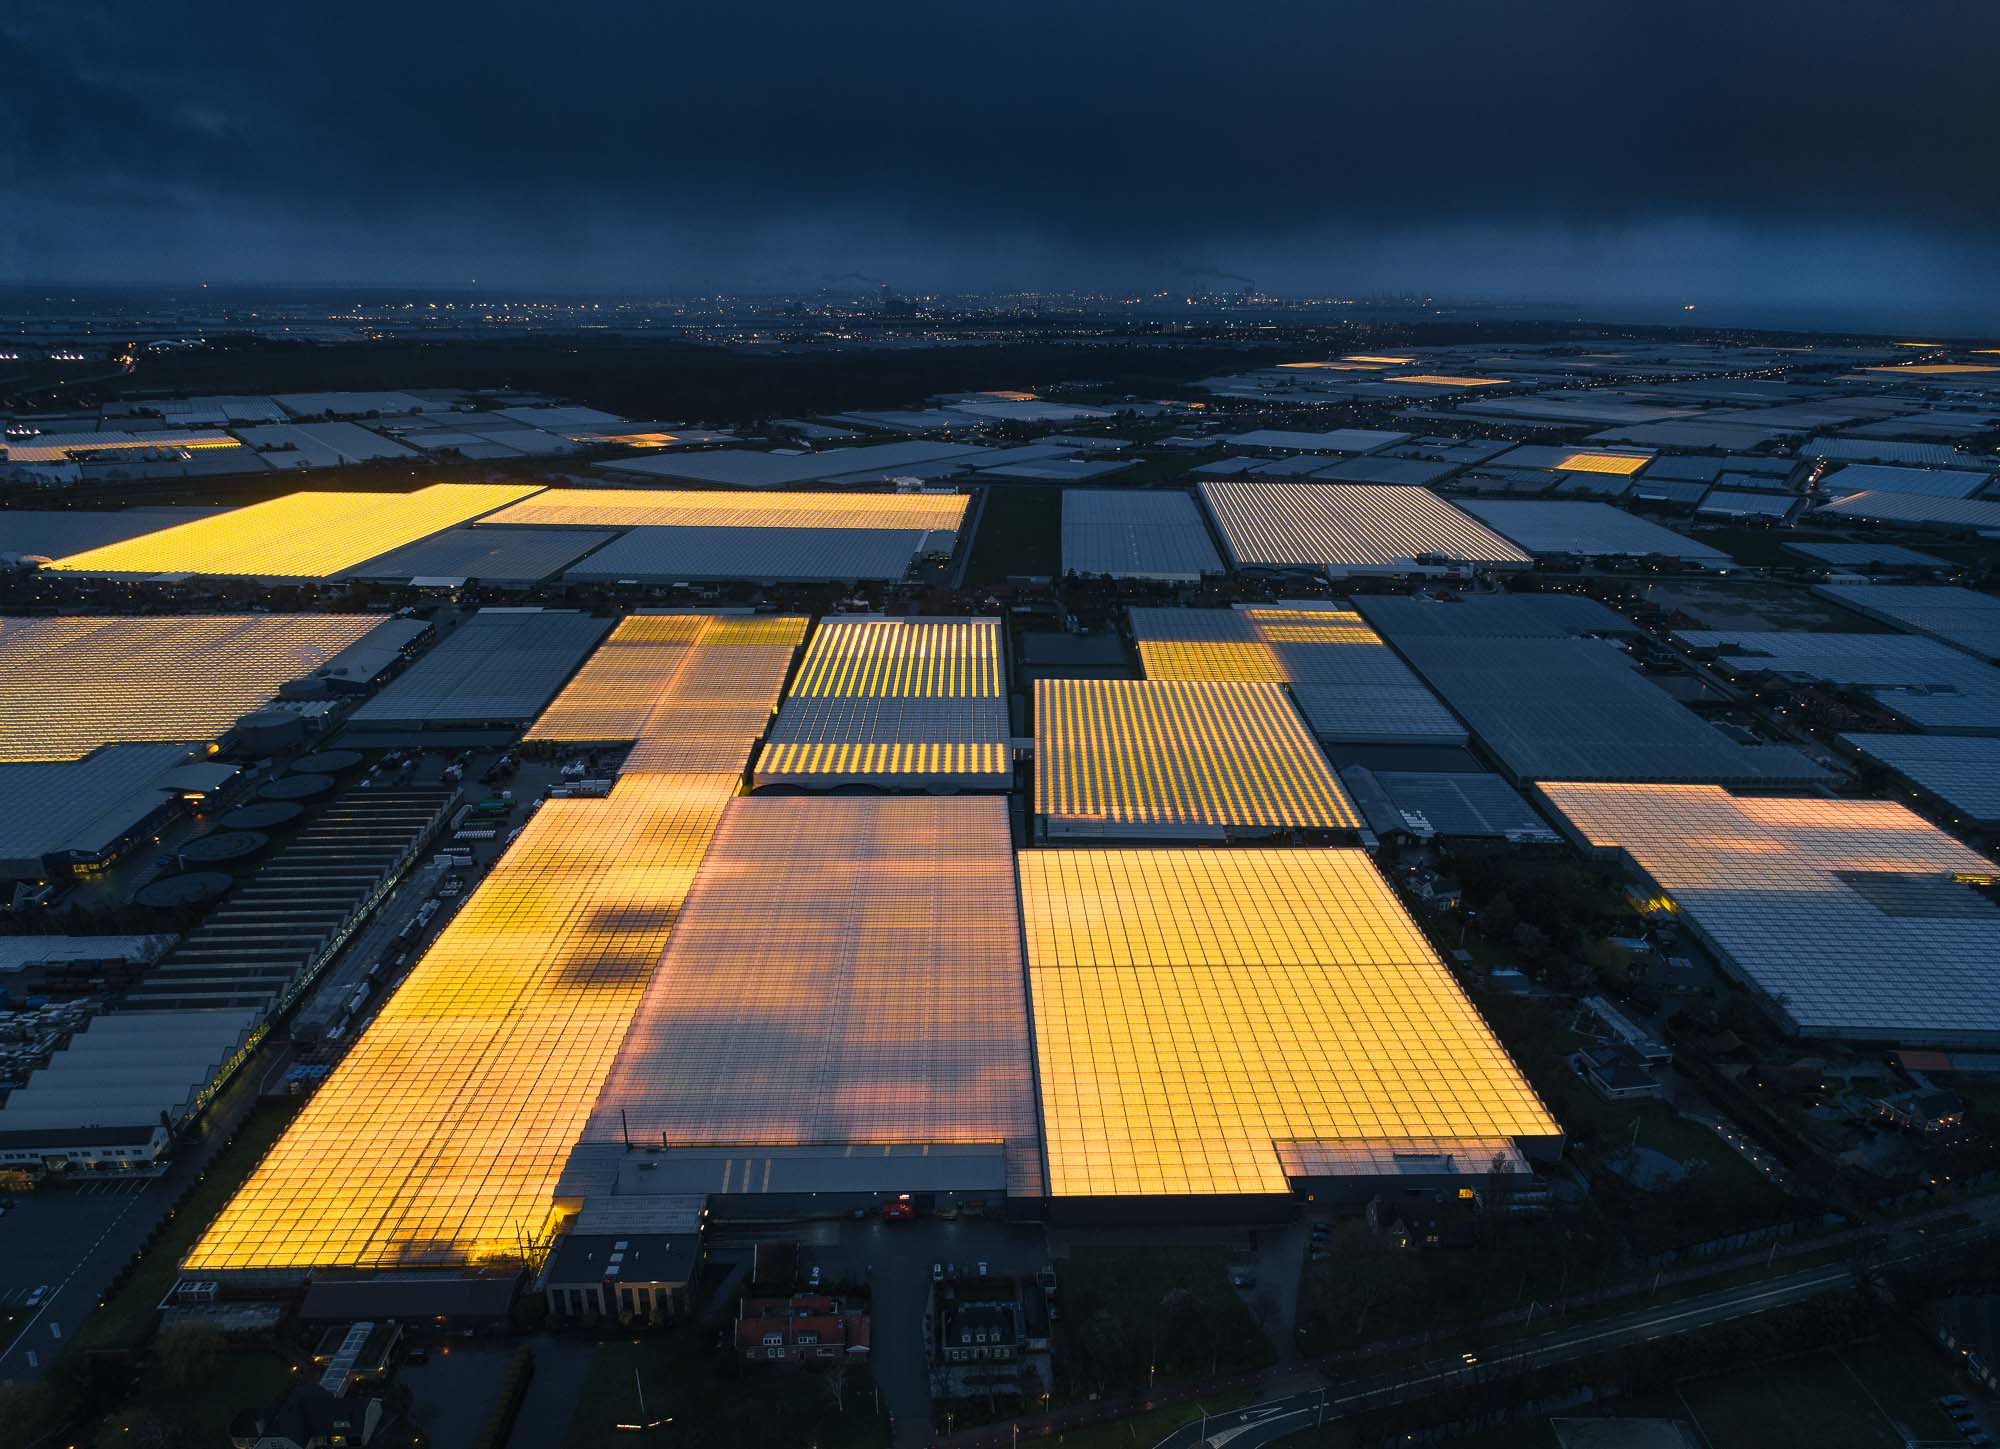
\includegraphics[width=15cm]{images/greenhousehegen.jpg}
    \caption{Netherlands' greenhouses with controlled environment agriculture - Tom Hegen (2019).}
    \label{fig:my_label}
\end{figure}
The transparent roofs with the huge amount of light make these greenhouses some of the brightest places on Earth. This kind of greenhouse can also be found outside Russia because all countries with high latitudes need to compensate for the lack of daylight, especially during the winter. To my knowledge, greenhouses never appear in the literature, even though it is a significant problem that needs to be addressed when dealing with night-time lights for economic applications. In 2021, the total light emitted by Russia cleaned by these two phenomena was about 20\% less than the un-cleaned imagery. A vast difference that, however, seems to be extremely invasive for Russia only. In other European countries, this phenomenon is much more limited. In Italy, for example, such outliers cannot be observed, not even in Spain, France and Germany. The only exception is the Netherlands, which has several greenhouses of the same Russian technology, albeit in smaller quantities.
Concerning gas flares, on the other hand, I found no outliers in Europe with the same Russian magnitude. On the contrary north African countries, endowed with well-known oil deposits, are full of them. 

Dealing with these outliers raises some critical economic questions. Greenhouses and gas flares enter directly into the GDP count. It is, therefore, questionable whether it is correct to eliminate or keep them. However, it is unrealistic to think that a pipeline vent in Siberia that emits as much light as an average European metropolis has the same impact on GDP. Therefore, I decided to clean the data from outliers but keep the original data, which will be compared on the following pages. 

\subsection{Outlier Removal strategies}

Several strategies are adopted to deal with outliers:
\begin{enumerate}
    \item Spatial correction: the algorithm checks each pixel and compares it with the surrounding area, usually $3\times3$ or $5\times5$ pixels. If the value of the pixel is several orders of magnitude higher than the average of the surrounding area, the pixel is recognised as an outlier and is removed
    \item Statistical correction: a predetermined percentile of the data distribution is removed. (For data from Russia, tests suggest the removal of the 0.001 tail)
    \item Manual correction: By looking at the values of cities and the central infrastructure of a country (airports, first of all), it is possible to derive a maximum threshold beyond which all other data are outliers. As far as Russia is concerned, the maximum value observed in cities is less than 500, while all values above are greenhouses or gas flares.
\end{enumerate}

For reasons of computational power, in this thesis, I will use the third approach since it appears to be sufficient. Moreover, power and RAM at a server level are required to manipulate this type of data.
%*****************************************
%*****************************************
%*****************************************
%*****************************************
%*****************************************
%\include{multiToC} % <--- just debug stuff, ignore for your documents
% ********************************************************************
% Backmatter
%*******************************************************
\appendix
%\renewcommand{\thechapter}{\alph{chapter}}
\cleardoublepage
%\part{Appendix}
%%********************************************************************
% Appendix
%*******************************************************
% If problems with the headers: get headings in appendix etc. right
%\markboth{\spacedlowsmallcaps{Appendix}}{\spacedlowsmallcaps{Appendix}}
\chapter{Appendix Test}
Lorem ipsum at nusquam appellantur his, ut eos erant homero
concludaturque. Albucius appellantur deterruisset id eam, vivendum
partiendo dissentiet ei ius. Vis melius facilisis ea, sea id convenire
referrentur, takimata adolescens ex duo. Ei harum argumentum per. Eam
vidit exerci appetere ad, ut vel zzril intellegam interpretaris.
\graffito{More dummy text.}

%Errem omnium ea per, pro congue populo ornatus cu, ex qui dicant
%nemore melius. No pri diam iriure euismod. Graecis eleifend
%appellantur quo id. Id corpora inimicus nam, facer nonummy ne pro,
%kasd repudiandae ei mei. Mea menandri mediocrem dissentiet cu, ex
%nominati imperdiet nec, sea odio duis vocent ei. Tempor everti
%appareat cu ius, ridens audiam an qui, aliquid admodum conceptam ne
%qui. Vis ea melius nostrum, mel alienum euripidis eu.

\section{Appendix Section Test}
Test: \autoref{tab:moreexample} (This reference should have a 
lowercase, small caps \spacedlowsmallcaps{A} if the option 
\texttt{floatperchapter} is activated, just as in the table itself
 $\rightarrow$ however, this does not work at the moment.)

\begin{table}[h]
    \myfloatalign
  \begin{tabularx}{\textwidth}{Xll} \toprule
    \tableheadline{labitur bonorum pri no} & \tableheadline{que vista}
    & \tableheadline{human} \\ \midrule
    fastidii ea ius & germano &  demonstratea \\
    suscipit instructior & titulo & personas \\
    %postulant quo & westeuropee & sanctificatec \\
    \midrule
    quaestio philosophia & facto & demonstrated \\
    %autem vulputate ex & parola & romanic \\
    %usu mucius iisque & studio & sanctificatef \\
    \bottomrule
  \end{tabularx}
  \caption[Autem usu id]{Autem usu id.}
  \label{tab:moreexample}
\end{table}

%Nulla fastidii ea ius, exerci suscipit instructior te nam, in ullum
%postulant quo. Congue quaestio philosophia his at, sea odio autem
%vulputate ex. Cu usu mucius iisque voluptua. Sit maiorum propriae at,
%ea cum primis intellegat. Hinc cotidieque reprehendunt eu nec. Autem
%timeam deleniti usu id, in nec nibh altera.




\section{Another Appendix Section Test}
Equidem detraxit cu nam, vix eu delenit periculis. Eos ut vero
constituto, no vidit propriae complectitur sea. Diceret nonummy in
has, no qui eligendi recteque consetetur. Mel eu dictas suscipiantur,
et sed placerat oporteat. At ipsum electram mei, ad aeque atomorum
mea. There is also a useless Pascal listing below: \autoref{lst:useless}.

\begin{lstlisting}[float=b,language=Pascal,frame=tb,caption={A floating example (\texttt{listings} manual)},label=lst:useless]
for i:=maxint downto 0 do
begin
{ do nothing }
end;
\end{lstlisting}

%Ei solet nemore consectetuer nam. Ad eam porro impetus, te choro omnes
%evertitur mel. Molestie conclusionemque vel at, no qui omittam
%expetenda efficiendi. Eu quo nobis offendit, verterem scriptorem ne
%vix.


%********************************************************************
% Other Stuff in the Back
%*******************************************************
\cleardoublepage%********************************************************************
% Bibliography
%*******************************************************
% work-around to have small caps also here in the headline
\manualmark
\markboth{\spacedlowsmallcaps{\bibname}}{\spacedlowsmallcaps{\bibname}} % work-around to have small caps also
%\phantomsection 
\refstepcounter{dummy}
\addtocontents{toc}{\protect\vspace{\beforebibskip}} % to have the bib a bit from the rest in the toc
\addcontentsline{toc}{chapter}{\tocEntry{\bibname}}
\label{app:bibliography}
\printbibliography

%\cleardoublepage%*******************************************************
% Declaration
%*******************************************************
\refstepcounter{dummy}
\pdfbookmark[0]{Declaration}{declaration}
\chapter*{Declaration}
\thispagestyle{empty}
Put your declaration here.
\bigskip
 
\noindent\textit{\myLocation, \myTime}

\smallskip

\begin{flushright}
    \begin{tabular}{m{5cm}}
        \\ \hline
        \centering\myName \\
    \end{tabular}
\end{flushright}

%\cleardoublepage\pagestyle{empty}

\hfill

\vfill


\pdfbookmark[0]{Colophon}{colophon}
\section*{Colophon}
This document was typeset using the typographical look-and-feel \texttt{classicthesis} developed by Andr\'e Miede. 
The style was inspired by Robert Bringhurst's seminal book on typography ``\emph{The Elements of Typographic Style}''. 
\texttt{classicthesis} is available for both \LaTeX\ and \mLyX: 
\begin{center}
\url{https://bitbucket.org/amiede/classicthesis/}
\end{center}
Happy users of \texttt{classicthesis} usually send a real postcard to the author, a collection of postcards received so far is featured here: 
\begin{center}
\url{http://postcards.miede.de/}
\end{center}
 
\bigskip

\noindent\finalVersionString

%Hermann Zapf's \emph{Palatino} and \emph{Euler} type faces (Type~1 PostScript fonts \emph{URW
%Palladio L} and \emph{FPL}) are used. The ``typewriter'' text is typeset in \emph{Bera Mono}, 
%originally developed by Bitstream, Inc. as ``Bitstream Vera''. (Type~1 PostScript fonts were made 
%available by Malte Rosenau and
%Ulrich Dirr.)

%\paragraph{note:} The custom size of the textblock was calculated
%using the directions given by Mr. Bringhurst (pages 26--29 and
%175/176). 10~pt Palatino needs  133.21~pt for the string
%``abcdefghijklmnopqrstuvwxyz''. This yields a good line length between
%24--26~pc (288--312~pt). Using a ``\emph{double square textblock}''
%with a 1:2 ratio this results in a textblock of 312:624~pt (which
%includes the headline in this design). A good alternative would be the
%``\emph{golden section textblock}'' with a ratio of 1:1.62, here
%312:505.44~pt. For comparison, \texttt{DIV9} of the \texttt{typearea}
%package results in a line length of 389~pt (32.4~pc), which is by far
%too long. However, this information will only be of interest for
%hardcore pseudo-typographers like me.%
%
%To make your own calculations, use the following commands and look up
%the corresponding lengths in the book:
%\begin{verbatim}
%    \settowidth{\abcd}{abcdefghijklmnopqrstuvwxyz}
%    \the\abcd\ % prints the value of the length
%\end{verbatim}
%Please see the file \texttt{classicthesis.sty} for some precalculated 
%values for Palatino and Minion.
%
%    \settowidth{\abcd}{abcdefghijklmnopqrstuvwxyz}
%    \the\abcd\ % prints the value of the length





% ********************************************************************
% Game Over: Restore, Restart, or Quit?
%*******************************************************
\end{document}
% ********************************************************************
